\chapter{Complex Networks Experiments}
\label{chap:Four}

\section{Introduction}
In this chapter, an additional experiment on the spatial topology of the IPD
is performed using complex networks. The spatial tournaments will be created using
three different methods. The methods will be explained and the network topologies produced by them
discussed. Followed, by an analysis on the data, including classification methods
based on cooperating ratio, network connectivity and clustering. The cooperating
ratio is a concept provided by the Axelrod-Python library and is computed
by dividing the number of times a strategy cooperated against the number of turns
in a single tournament. Furthermore, regression models are built for the normalized rank.

The issues raised in~\autoref{chap:Three}, will be addessed in the current chapter,
altering various approaches. For example, median ranking is introduced as a more
accurate performance measure and the round robin in treated as a spatial tournament
of a complete topology.

\section{Networks and Methods}
\label{sub:methods}
A complex network is a graph with non-trivial topological features;
features that can not occur in networks such as the ones studied in ~\autoref{chap:Three}.
Such features include, a heavy tail in the degree distribution, a high
clustering coefficient, and hierarchical structure. Complex networks are commonly
used to study computer networks, technological networks and social networks~\cite{VanDerHofstad2009}.

They will also be used in the experiment conducted in this dissertation. Three
different methods, for creating such networks and using them as topologies, have
been used. Each of the methods adopts one of the following models to produce the
required graphs.

\begin{itemize}
	\item Watts Strogatz, a model for generating graphs with small-world properties\cite{Watts1998}
	\item Erd\"{o}s R\'{e}nyi, a model for generating random graphs~\cite{Erdos1959}
	\item Complete graph, a graph with the properties of a round robin topology\cite{Harris2010}
\end{itemize}

Each of the models has a different set of parameters and each of the methods
produce different number of networks. The structure of each method is analyzed in
the following subsection.

\subsection{Methods Structure}
\label{sub:experiments-structure}
\subsubsection{Method for small world networks}

In the method of small world networks, the Watts Strogatz model has been used
for generating the required graphs.
The Watts Strogatz model, was proposed by D. Watss and S. Strogatz,
in their work in 1998~\cite{Watts1998}. Their work has been focused on the reproduction
of a network, which interpolated between a regular and a random network.
To achieve this, they considered a random rewiring procedure with the following
rules:

\begin{itemize}
	\item start from a ring lattice with \(n\) vertices and \(k\) the initial edges per vertex
	\item rewire each edges with a probability of \(p\)
\end{itemize}

For the computational approach, \texttt{Networkx}~\cite{networkx} Python library provides the
\texttt{watts\_strogatz\_graph} function. Documentation can be found here:
\url{https://networkx.github.io/documentation/development/reference/generated/networkx.generators.random_graphs.watts_strogatz_graph.html#networkx.generators.random_graphs.watts_strogatz_graph}.
The method's structure is explained
in the Algorithm~\ref{alg:small-world-method}. As shown, the tournament size is
deterministic, ranging for 2 to 50. The initial edges per vertex, ranges from 2
to tournament size minus 1. The random selection of players is repeated 100 times
and each set of selected players is being shuffled for 10 repetitions.

\begin{algorithm}
	\caption{Method for small world networks}\label{alg:small-world-method}
	\begin{algorithmic}
		\Procedure{Small World}{}
		\BState \emph{loop}:
		\For {$\textit{tournament.size} \gets \textit{ 2 to 50}$}
		\For {$\textit{initial.edges.per.vertex} \gets \textit{1 to tournament.size-1}$}
		\For {$\textit{i} \gets \textit{ 0 to 10}$}
		\State $player \gets \textit{random.strategies}$.
		\For {$p \gets \textit{0 to 10}$}
		\State $G \gets \textit{create.watts.strogatz.graph}$.
		\State $edges \gets \textit{G.egdes}$
		\State $results \gets \textit{play.tournament}$.
		\emph{loop}.
		\EndFor
		\EndFor
		\EndFor
		\EndFor
		\EndProcedure
	\end{algorithmic}
\end{algorithm}

\subsubsection{Method for random networks}
In the method of random networks, the desired networks have been produced using the
Erd\"{o}s R\'{e}nyi model.
The model is named after P. Erd\"{o}s and A. R\'{e}nyi, who introduced
the model in 1959~\cite{Erdos1959}. It generates a random graph of \(n\)
vertices and each of the possible edges with probability \(p\).

Similarly, \texttt{Networkx} library provides the function \texttt{binomial\_graph}
for generating such graphs. Documentation can be found here:
\url{https://networkx.github.io/documentation/development/reference/generated/networkx.generators.random_graphs.binomial_graph.html#networkx.generators.random_graphs.binomial_graph}.
Algorithm~\ref{random-method}, illustrate the structure of the method for random
networks. Similarly, the tournament size is not deterministic, instead it
ranges from 2 to 50. A 100 sets of random players are created, and shuffled,
for 10 repetitions.

\begin{algorithm}[H]
	\caption{Method for random networks}\label{random-method}
	\begin{algorithmic}
		\Procedure{Random}{}
		\BState \emph{loop}:
		\For {$\textit{tournament.size} \gets \textit{2 to 50}$}
		\For {$\textit{i} \gets \textit{0 to 100}$}
		\State $player \gets \textit{random.strategies}$.
		\For {$p \gets \textit{0 to 10}$}
		\State $G \gets \textit{create.erdos.renyi.graph}$.
		\State $edges \gets \textit{G.egdes}$
		\State $results \gets \textit{play.tournament}$.
		\emph{loop}.
		\EndFor
		\EndFor
		\EndFor
		\EndProcedure
	\end{algorithmic}
\end{algorithm}

\subsubsection{Method for complete networks}
The method for producing complete networks, uses the \texttt{complete\_graph} function
from the \texttt{Networkx} library:\url{https://networkx.github.io/documentation/development/reference/generated/networkx.generators.classic.complete_graph.html#networkx.generators.classic.complete_graph}
The structure of the method is illustrated by the Algorithm~\ref{complete-method}.

\begin{algorithm}
	\caption{Method for complete networks}\label{complete-method}
	\begin{algorithmic}
		\Procedure{Complete}{}
		\BState \emph{loop}:
		\For {$\textit{tournament.size} \gets \textit{2 to 50}$}
		\For {$\textit{i} \gets \textit{ 0 to 100}$}
		\State $player \gets \textit{random.strategies}$.
		\State $G \gets \textit{create.complete.graph}$.
		\State $edges \gets \textit{G.egdes}$
		\State $results \gets \textit{play.tournament}$.
		\emph{loop}.
		\EndFor
		\EndFor
		\EndProcedure
	\end{algorithmic}
\end{algorithm}

\section{Data generation}
The goal of this chapter is the observation of the strategies behavior when
participating in spatial tournaments of any given topology. Here only three
different types of complex networks will be used. Thus, the data set for this
chapter is a collection of data generated by using the three aforementioned
methods (~\autoref{sub:methods}). Executing these methods requires a high
computational power, considering that over a 1000 of tournaments are
simulated. Thus, they are executed in Raven.

Furthermore, Hierarchical Data Format (HDF5) was used as the file format.
HDF5 is a data model, library, and file format for storing and managing data~\cite{hdf5}.
Python offers an HDF5 binding and HDF5 has various advantages, fitted for the needs
of this chapter. For example, the large amounts of data will be easily stored
and the data can be access without loading them on memory making the analysis
faster.

In ~\autoref{preliminary-analysis}, a preliminary analysis on the individual results of each method
is performed. Followed, by in depth analysis to the whole data set in~\autoref{performance-analysis}.

\section{Preliminary Analysis}
\label{preliminary-analysis}
In this section, the outputs of the three methods are described individually.
Starting with an analysis on the networks attributes that have been produced as topologies,
following a preliminary analysis on the results of their given spatial tournaments.

\subsection{Network Analysis}
\label{sub:network-analysis}
The networks of each method are studied. As introduced in ~\autoref{sub:graph-theory}, the
connectivity and clustering concepts are summarized and reviewed. Due to the
size of experiments and time constraints, not all methods managed to
maximize their tournament sizes, as they have been described in~\autoref{sub:experiments-structure}.

More specifically, for the small world method, a total of 59051 graphs have
been created. The maximum number of nodes achieved is 13. Moreover, the
mean degree, has been 4.75. Thus indicating that
in most tournaments, the average number of neighbors per strategy was 4.
The maximum degree is equal to 12. Further,
the mean connectivity of the small world network is 3.40, the minimum is 0 and the maximum 9.
The clustering coefficient ranges from 0 to 1, with a mean of 0.48. A mean
of 0.48, for the clustering coefficients, indicates that strategies have a
neutral trend towards creating cliques (complete graphs).

\begin{table}[!hbtp]
	\centering
	\begin{adjustbox}{width=0.5\textwidth}
		\small
		\begin{tabular}{cccccccccc}
				\toprule
			\multicolumn{5}{|c|}{Small world Networks Summary Table}           \\ \hline
			     & connectivity & clustering & degree & nodes                  \\ \hline
			mean & 3.40         & 0.48       & 4.75   & 10.00                  \\ \hline
			std  & 2.37         & 0.33       & 2.65   & \multicolumn{1}{c}{-} \\ \hline
			min  & 0.00         & 0.00       & 1.00   & 3.00                   \\ \hline
			max  & 9.00         & 1.00       & 12.00  & 13.00                   \\ \bottomrule
		\end{tabular}
	\end{adjustbox}
	\caption{Small world summary table}
	\label{table:small-world-summary-table}
\end{table}

\newpage
Illustrating 59051 graphs for understanding the networks of the experiment, is
an impossible task. For this reason, the summary Table~\ref{table:small-world-summary-table}
has been used. Furthermore, six networks have been randomly selected and
displayer in Figure~\ref{fig:small_networks_illustration}. Mainly to get an idea
of the look of the networks in this method.

\begin{figure}[!hbtp]
	\centering
	\begin{subfigure}[t]{0.30\textwidth}
		\centering
		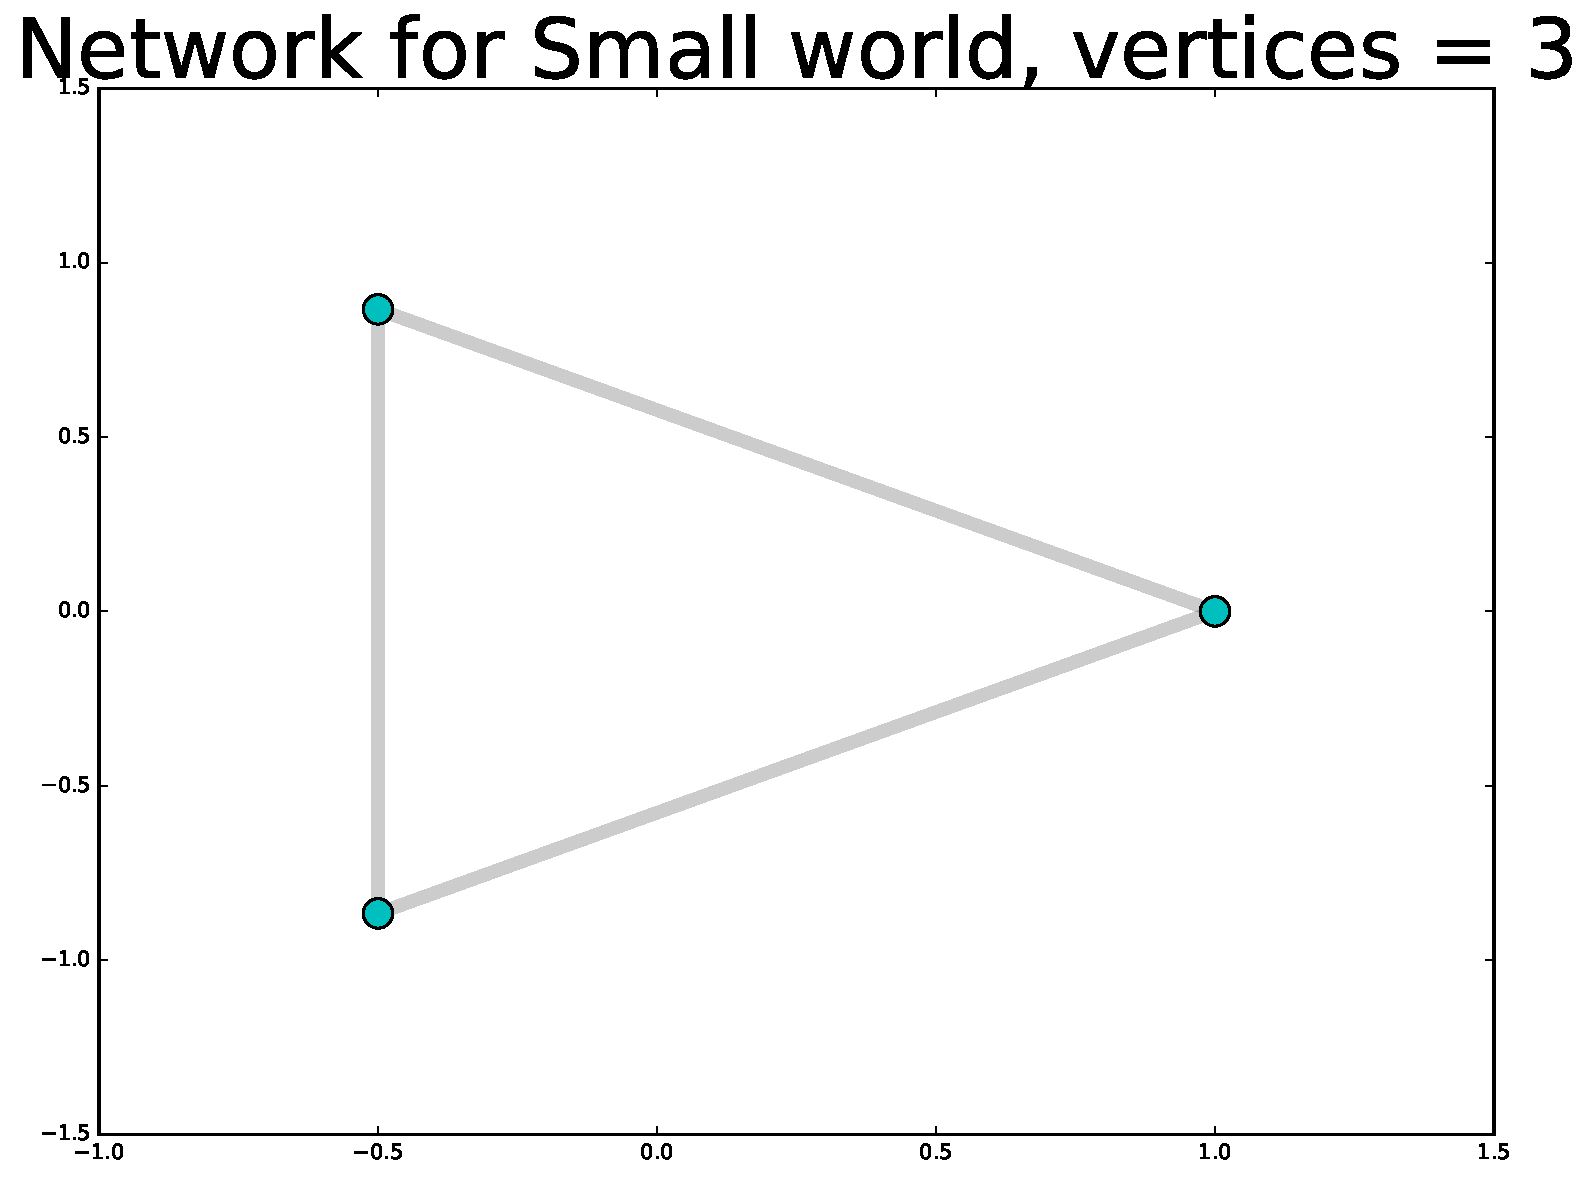
\includegraphics[width=\linewidth]{chapter-four/small__networks_3.pdf}
		\caption{Three nodes}
	\end{subfigure}
	\hfill
	\begin{subfigure}[t]{0.30\textwidth}\centering
		\centering
		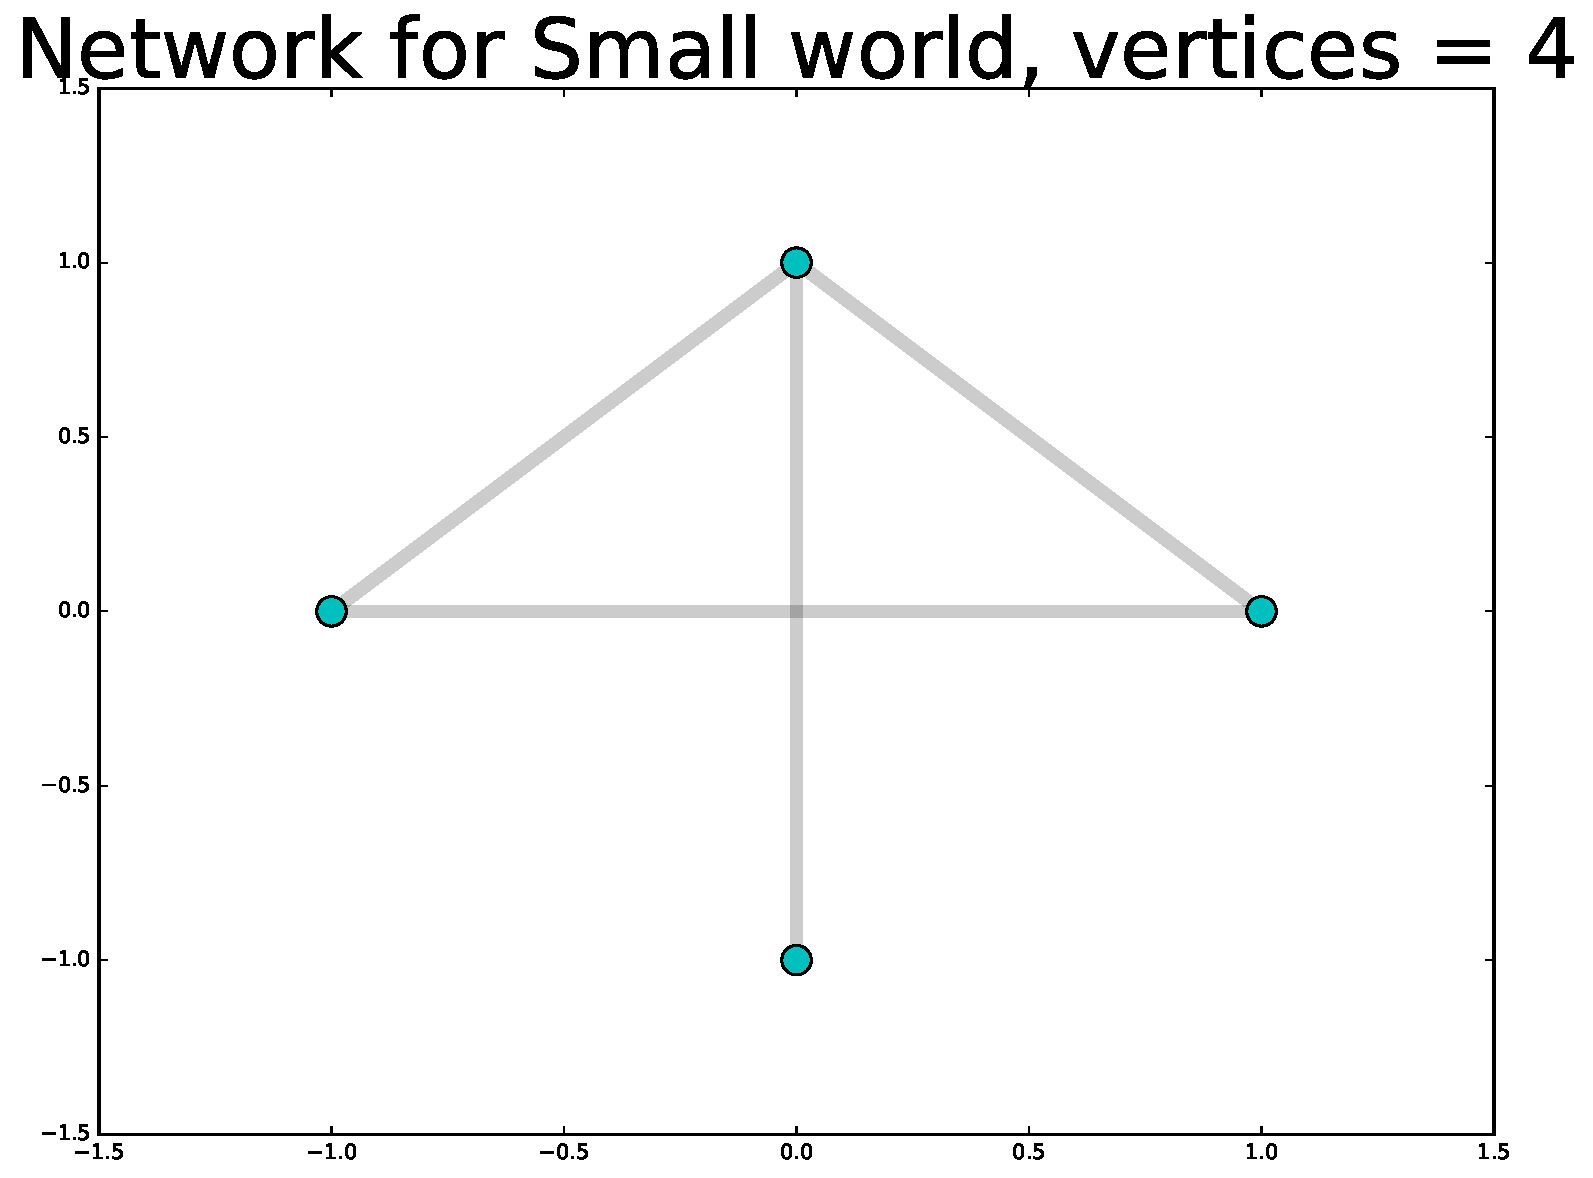
\includegraphics[width=\linewidth]{chapter-four/small__networks_4.pdf}
		\caption{Four nodes}
	\end{subfigure}
	\hfill
	\begin{subfigure}[t]{0.30\textwidth}\centering
		\centering
		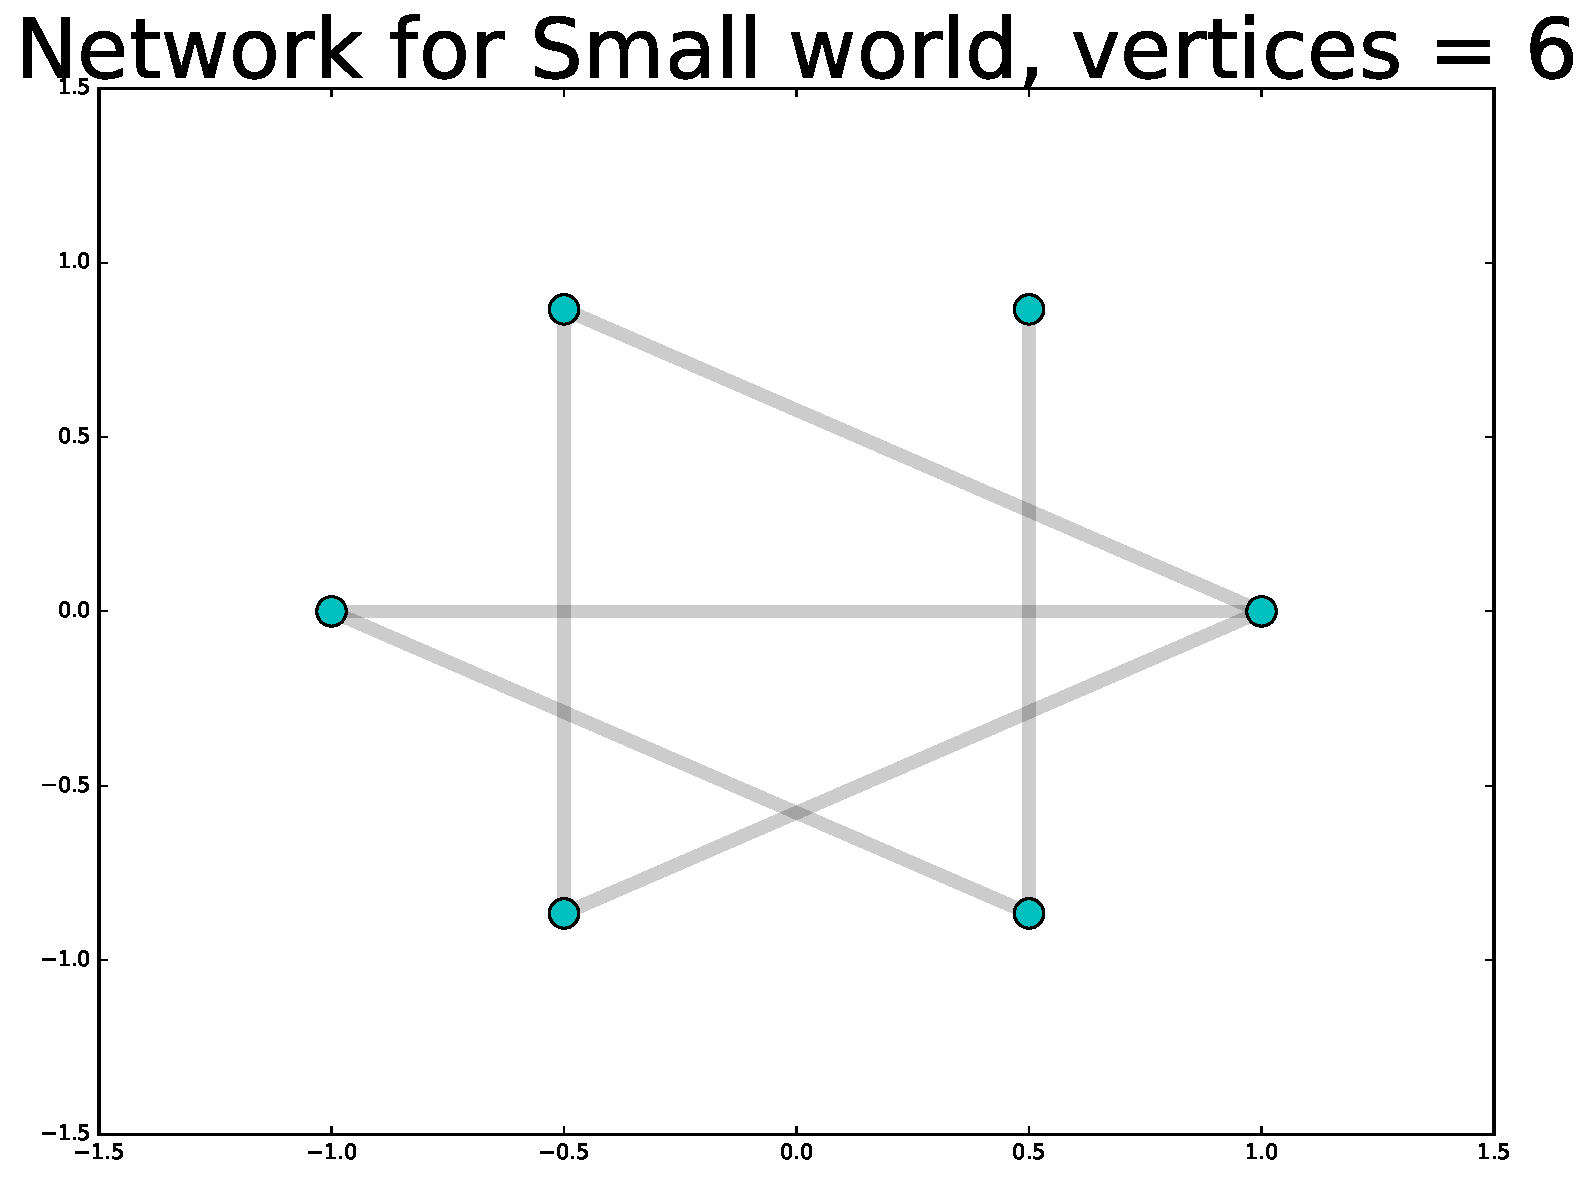
\includegraphics[width=\linewidth]{chapter-four/small__networks_6.pdf}
		\caption{Six nodes}
	\end{subfigure}
	\hfill
	\begin{subfigure}[t]{0.30\textwidth}\centering
		\centering
		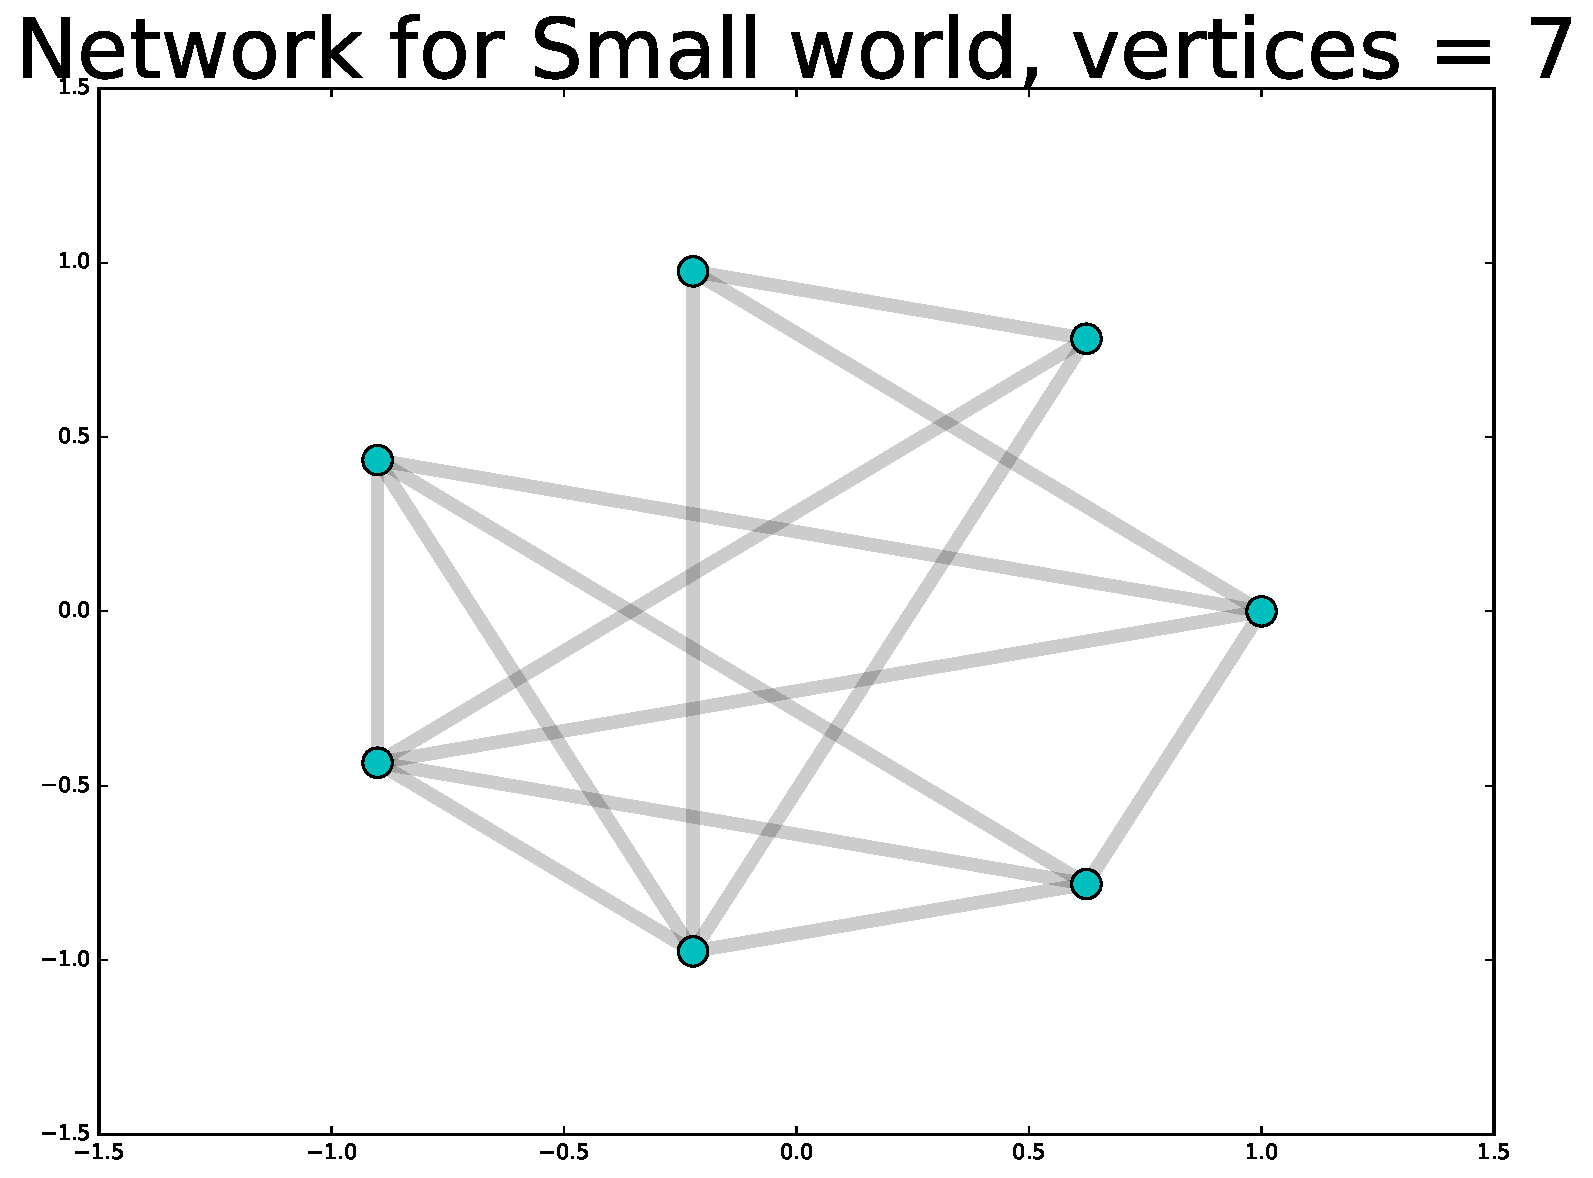
\includegraphics[width=\linewidth]{chapter-four/small__networks_7.pdf}
		\caption{Seven nodes}
	\end{subfigure}
	\hfill
	\begin{subfigure}[t]{0.30\textwidth}\centering
		\centering
		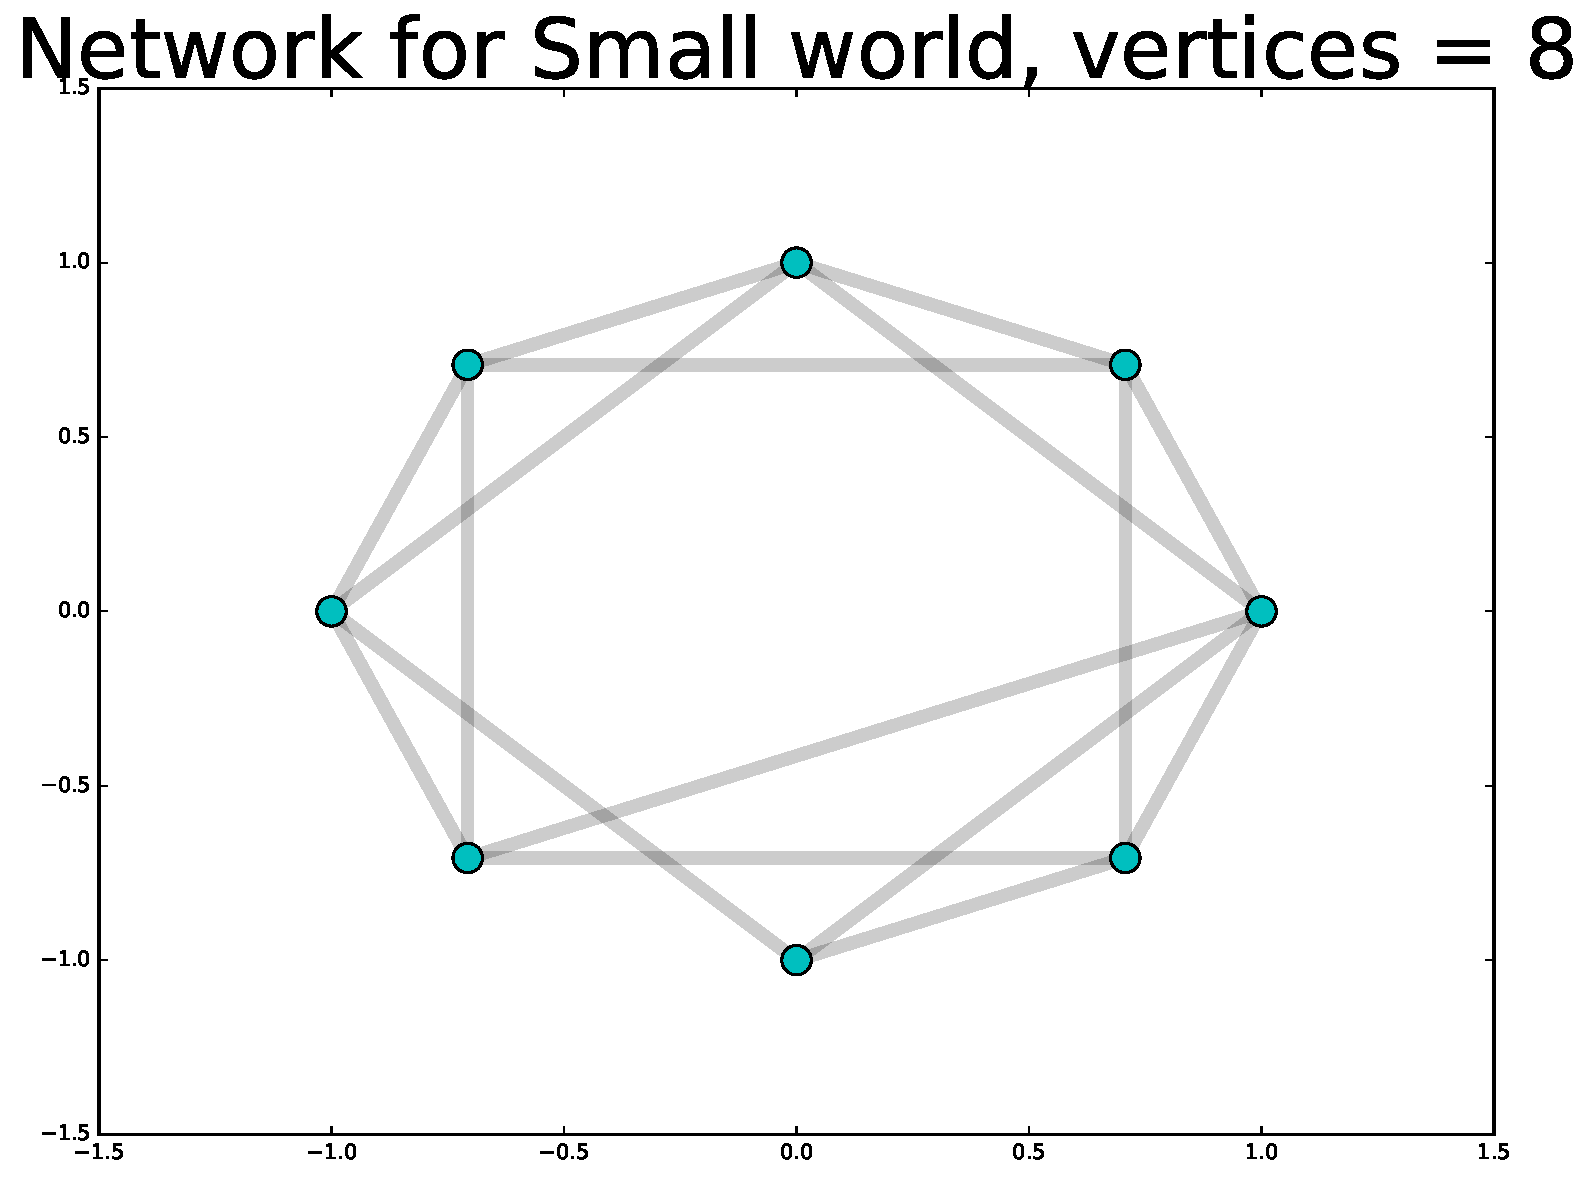
\includegraphics[width=\linewidth]{chapter-four/small__networks_8.pdf}
		\caption{Eight nodes}
	\end{subfigure}
	\hfill
	\begin{subfigure}[t]{0.30\textwidth}\centering
		\centering
		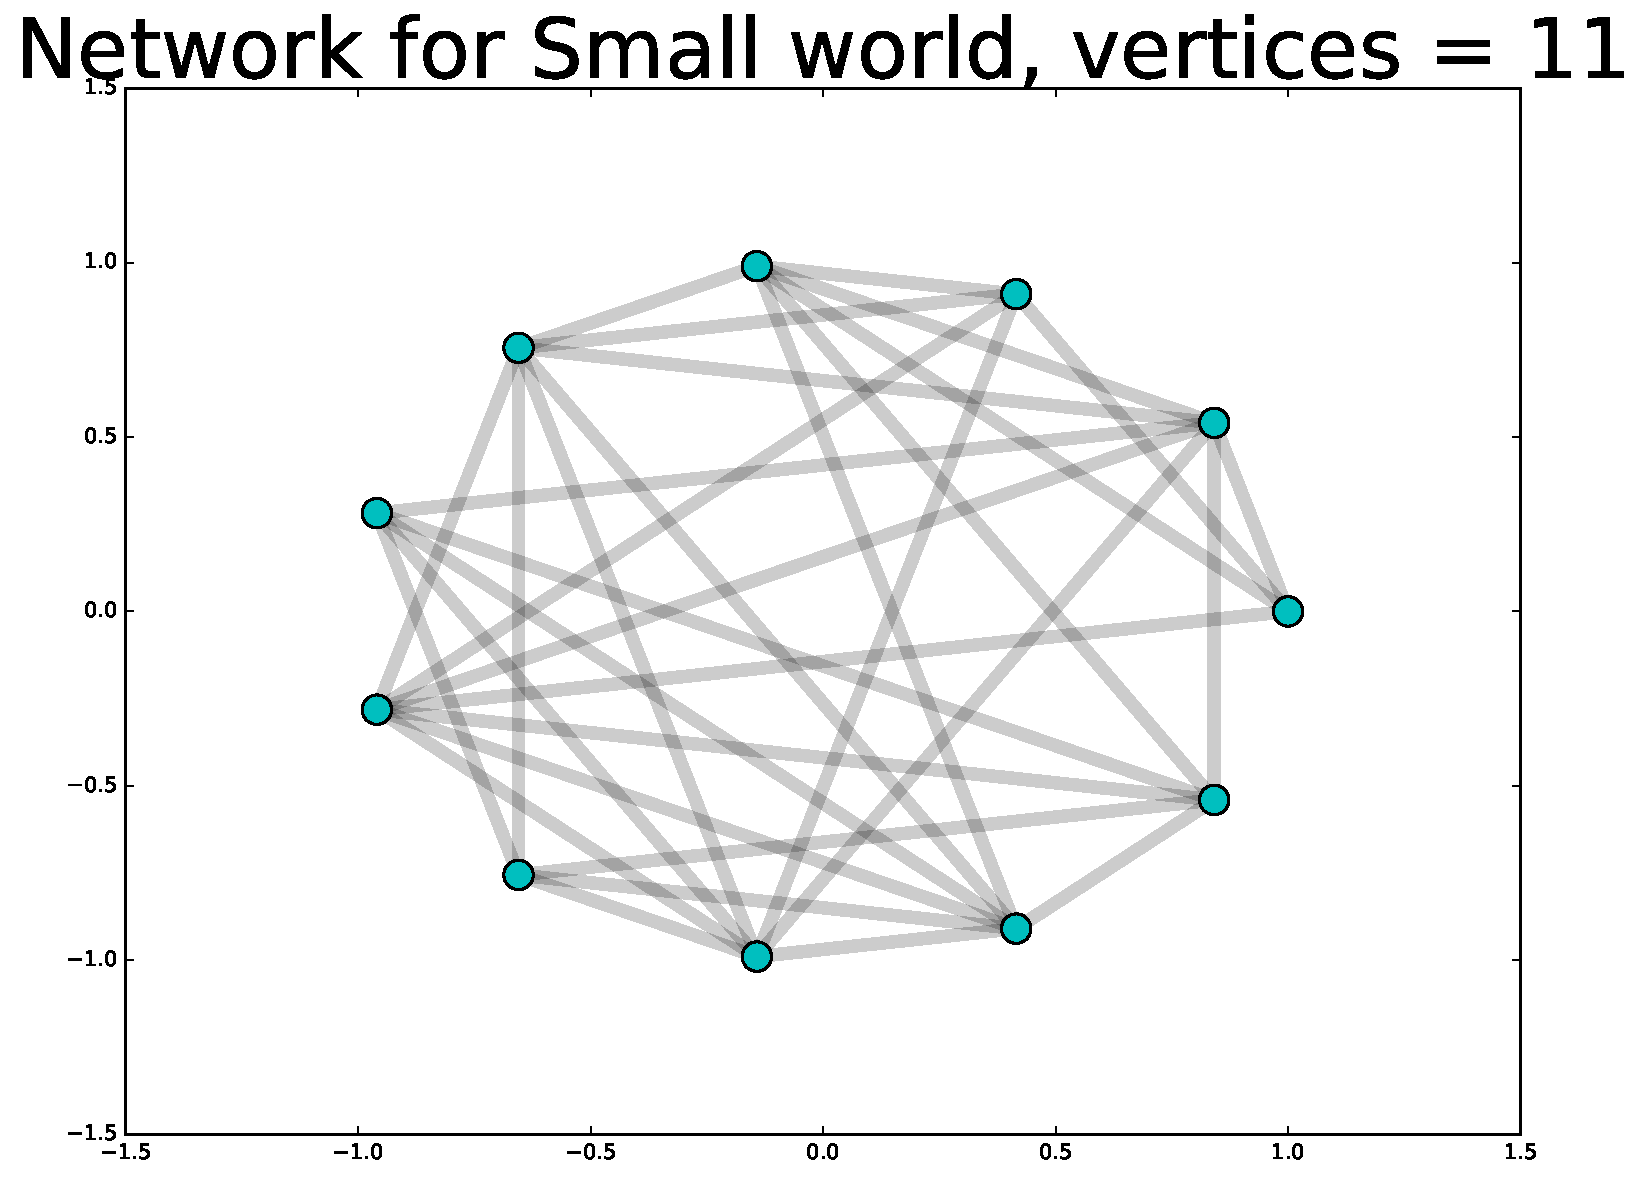
\includegraphics[width=\linewidth]{chapter-four/small__networks_11.pdf}
		\caption{Eleven nodes}
	\end{subfigure}
	\caption{Various Watss Strogatz networks}
	\label{fig:small_networks_illustration}
\end{figure}

Likewise for the random networks method. The experiment did not manage to
achieve the maximum tournament size that had been set. Instead, 21924 have been
created. As shown in Table~\ref{table:binomial-summary-table}, the mean number
of nodes of the experiments has been 20, the minimum 2 and the maximum 29. The
mean connectivity, of a random network, is approximately 8.26, the minimum
0.00 and maximum 28.00.

\begin{table}[H]
	\centering
	\begin{adjustbox}{width=0.5\textwidth}
		\small
		\begin{tabular}{cccccccccc}
				\toprule
			\multicolumn{5}{|c|}{Random Networks Summary Table}                       \\ \hline
			     & connectivity & clustering & degree & nodes                  \\ \hline
			mean & 8.26         & 0.60       & 11.22  & 19.80                  \\ \hline
			std  & 6.46         & 0.30       & 6.50   & \multicolumn{1}{c}{-} \\ \hline
			min  & 0.00         & 0.00       & 1.00   & 2.00                   \\ \hline
			max  & 28.00        & 1.00       & 28.00  & 29.00                  \\ \bottomrule
		\end{tabular}
	\end{adjustbox}
	\caption{Random summary table}
	\label{table:binomial-summary-table}
\end{table}

The clustering coefficient, of the random networks has a mean value of 0.60. The
mean node number is equal to 20 with a mean degree 11. Thus, in most of the
tournaments that occurred, the strategy had to compete with 11 of it's neighbors.
Once again, six random have been picked and are illustrated in Figure ~\ref{random_networks_illustration}.

\begin{figure}[H]
	\centering
	\begin{subfigure}[t]{0.30\textwidth}
		\centering
		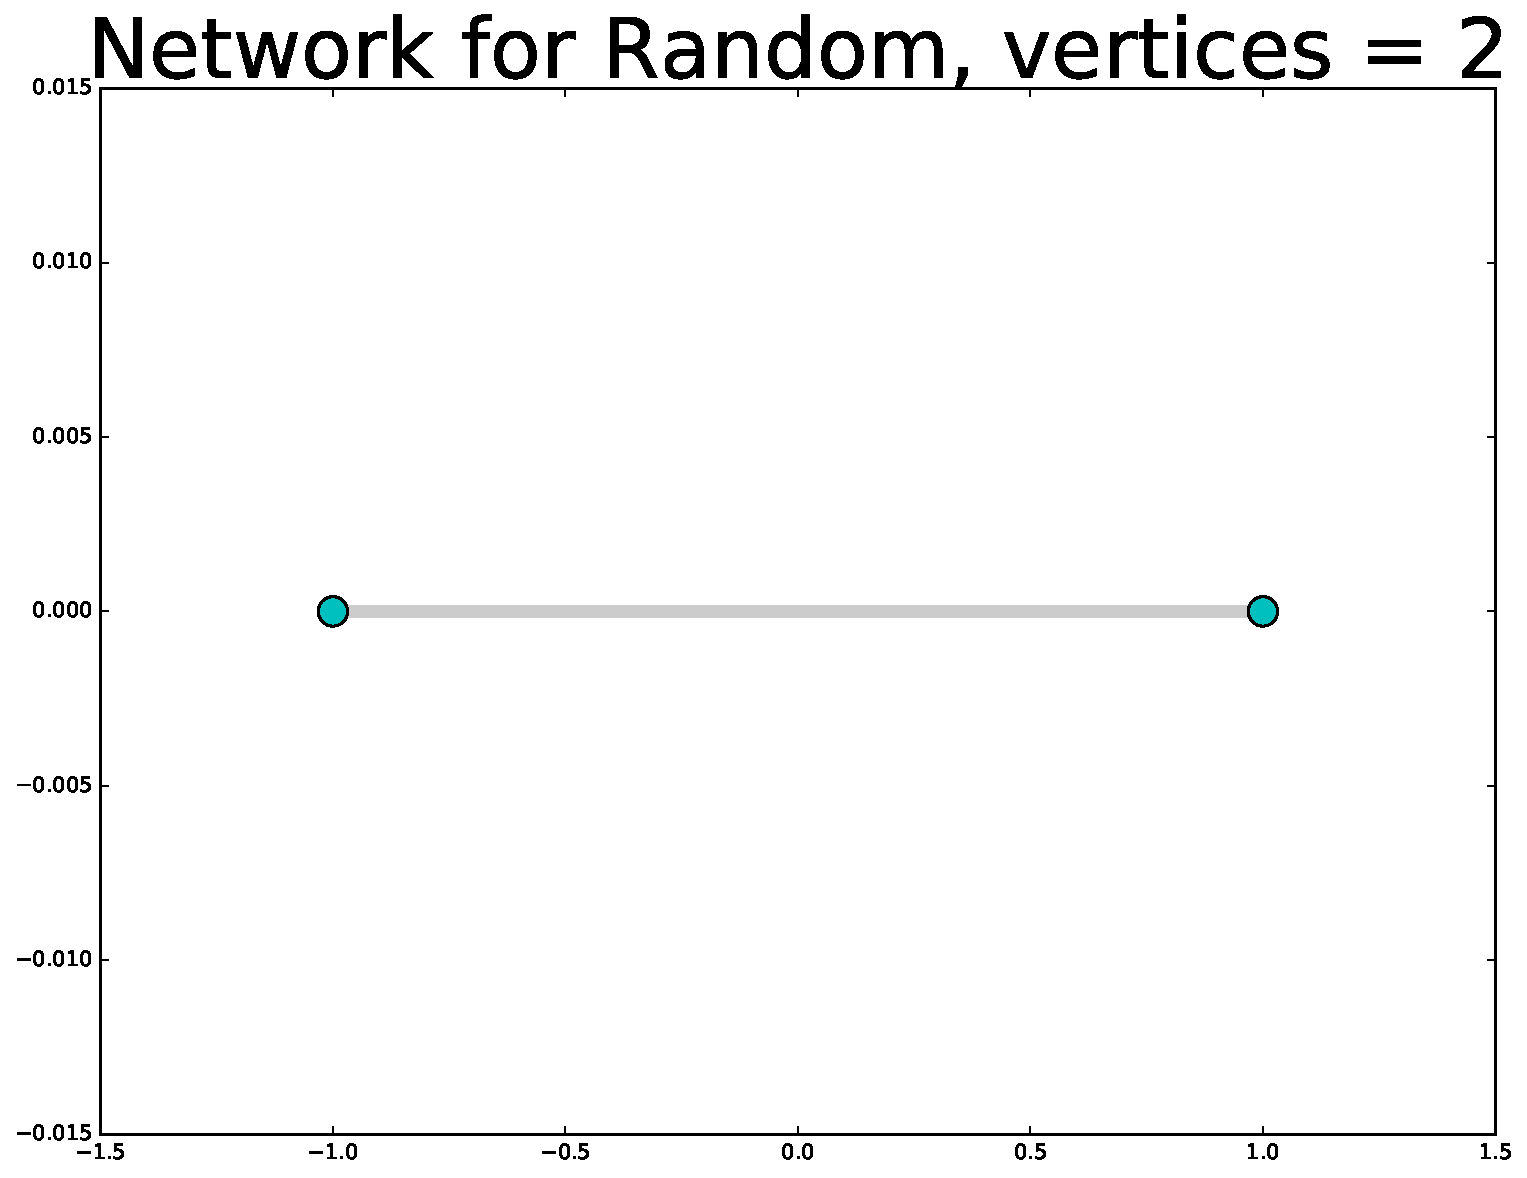
\includegraphics[width=\linewidth]{chapter-four/random_2.pdf}
		\caption{Two nodes}
	\end{subfigure}
	\hfill
	\begin{subfigure}[t]{0.30\textwidth}\centering
		\centering
		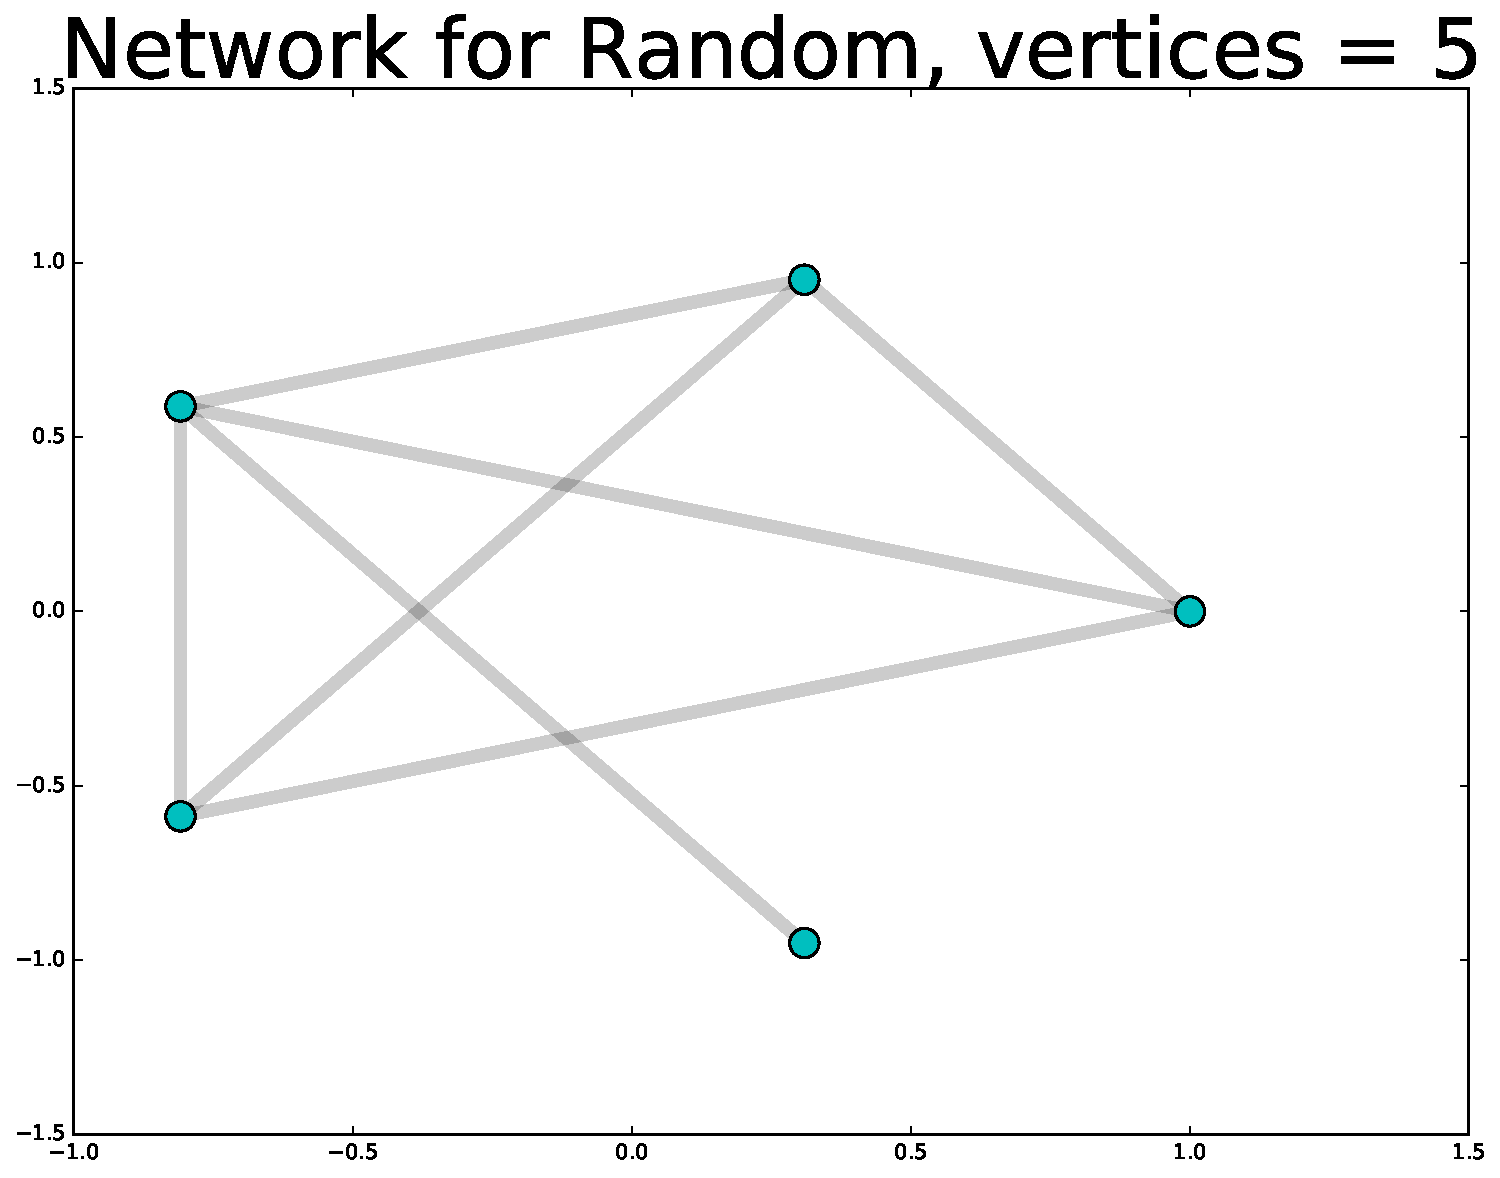
\includegraphics[width=\linewidth]{chapter-four/random_5.pdf}
		\caption{Five nodes}
	\end{subfigure}
	\hfill
	\begin{subfigure}[t]{0.30\textwidth}\centering
		\centering
		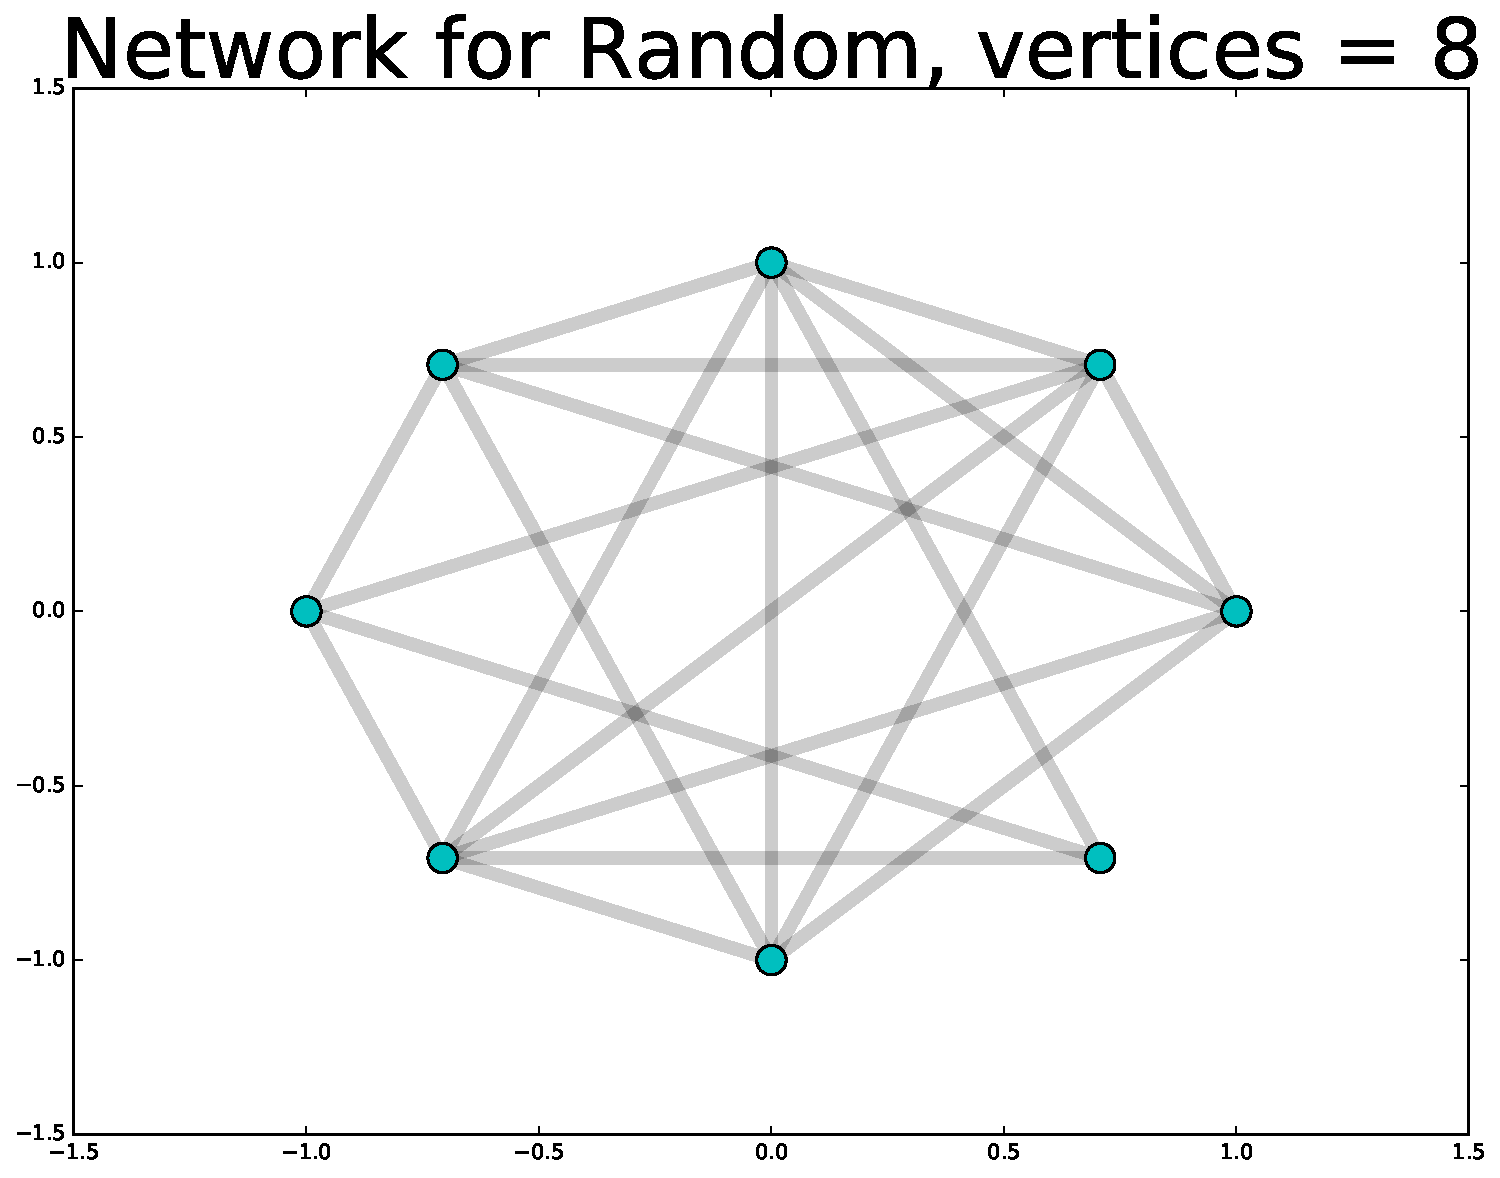
\includegraphics[width=\linewidth]{chapter-four/random_8.pdf}
		\caption{Eight nodes}
	\end{subfigure}
	\hfill
	\begin{subfigure}[t]{0.30\textwidth}\centering
		\centering
		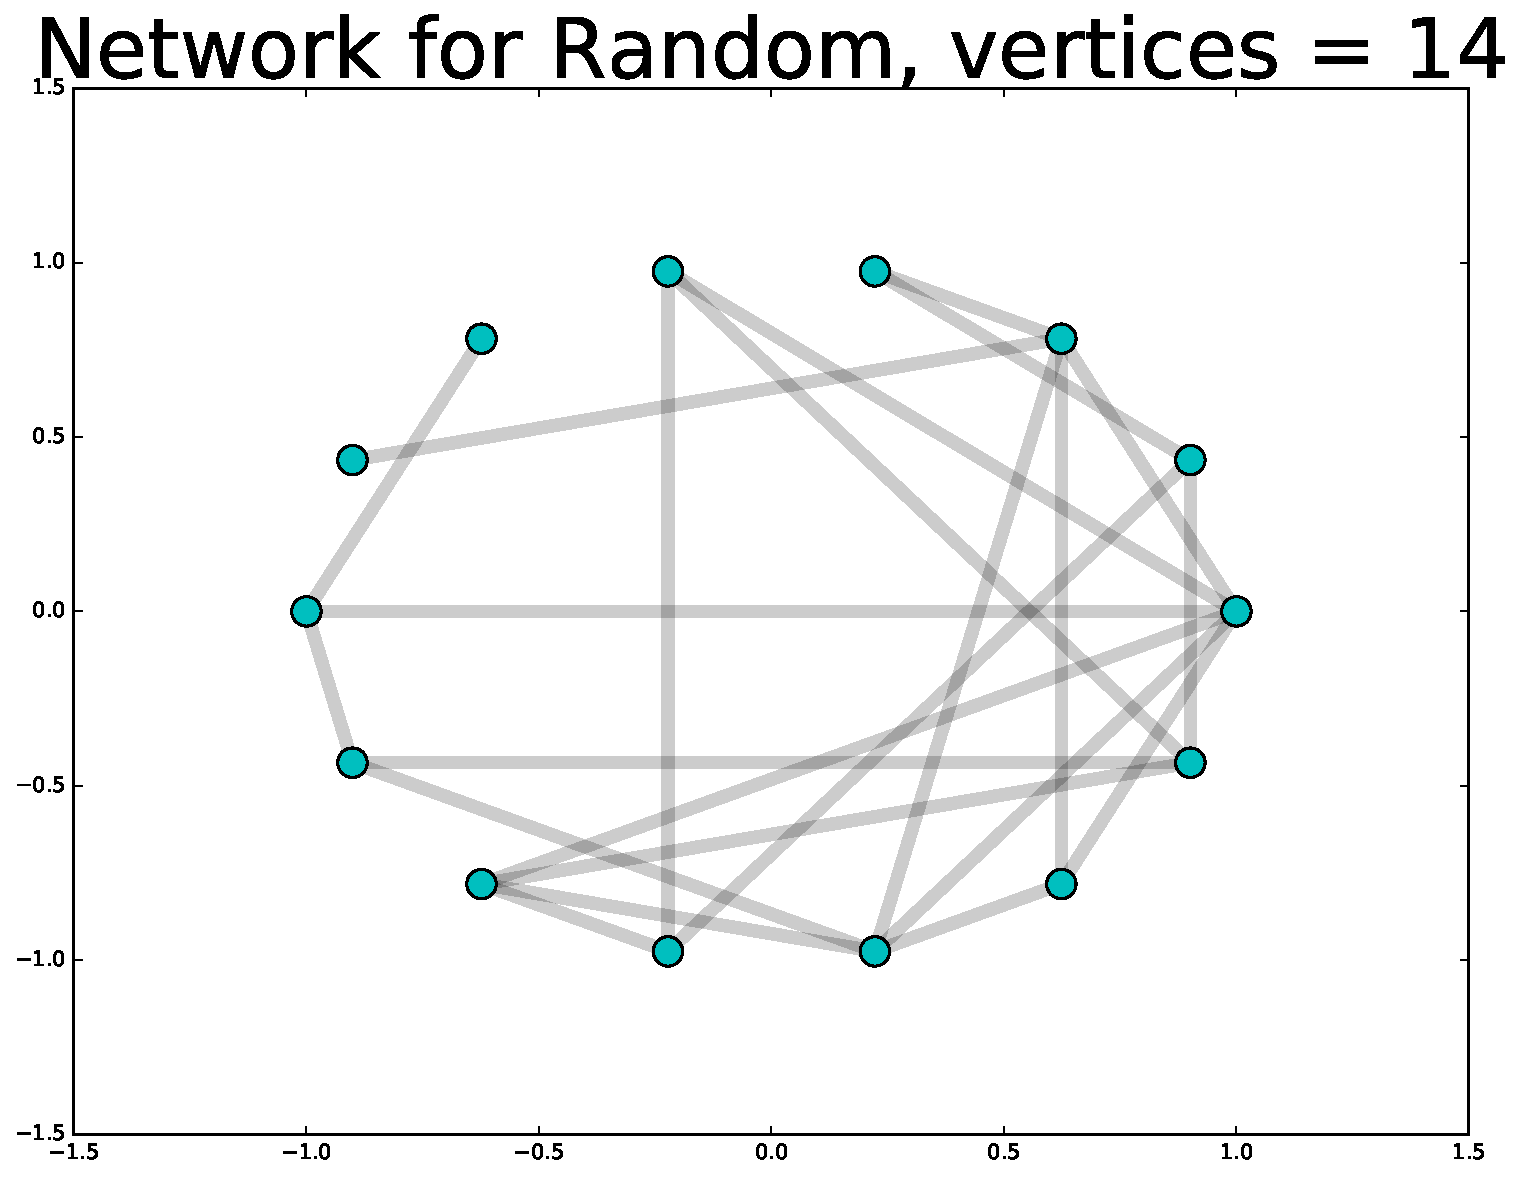
\includegraphics[width=\linewidth]{chapter-four/random_14.pdf}
		\caption{Fourteen nodes}
	\end{subfigure}
	\hfill
	\begin{subfigure}[t]{0.30\textwidth}\centering
		\centering
		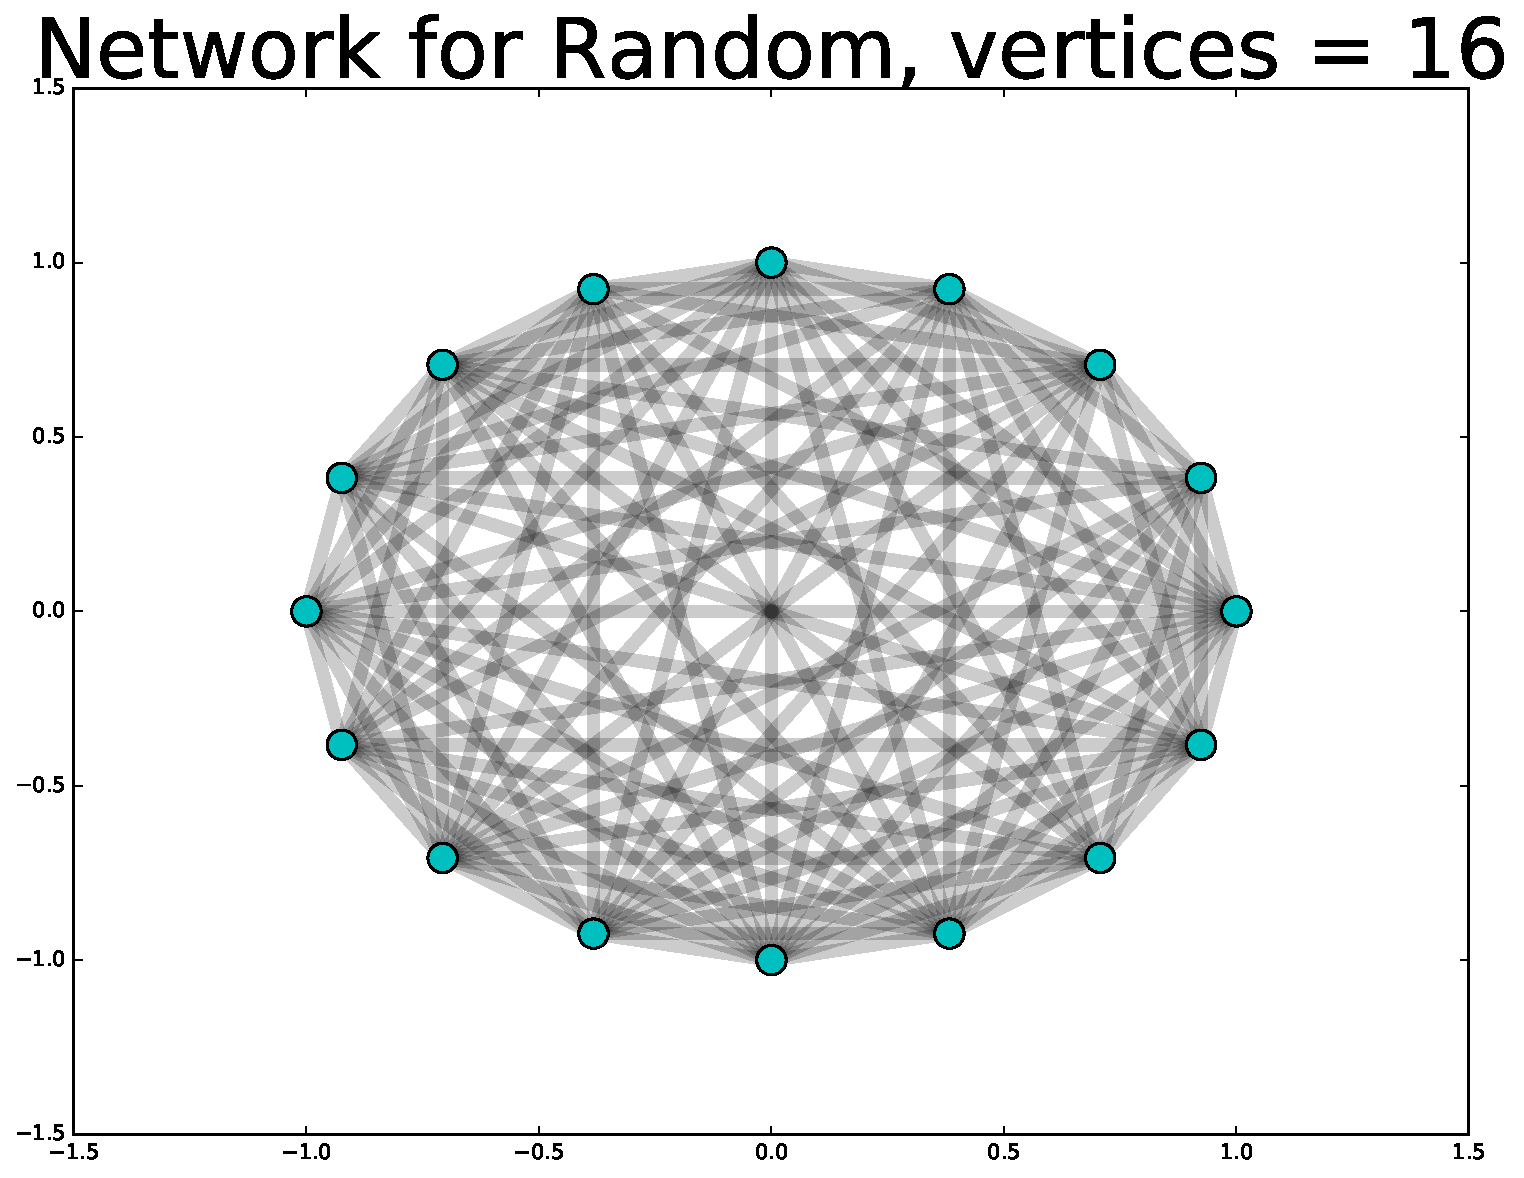
\includegraphics[width=\linewidth]{chapter-four/random_16.pdf}
		\caption{Sixteen nodes}
	\end{subfigure}
	\hfill
	\begin{subfigure}[t]{0.30\textwidth}\centering
		\centering
		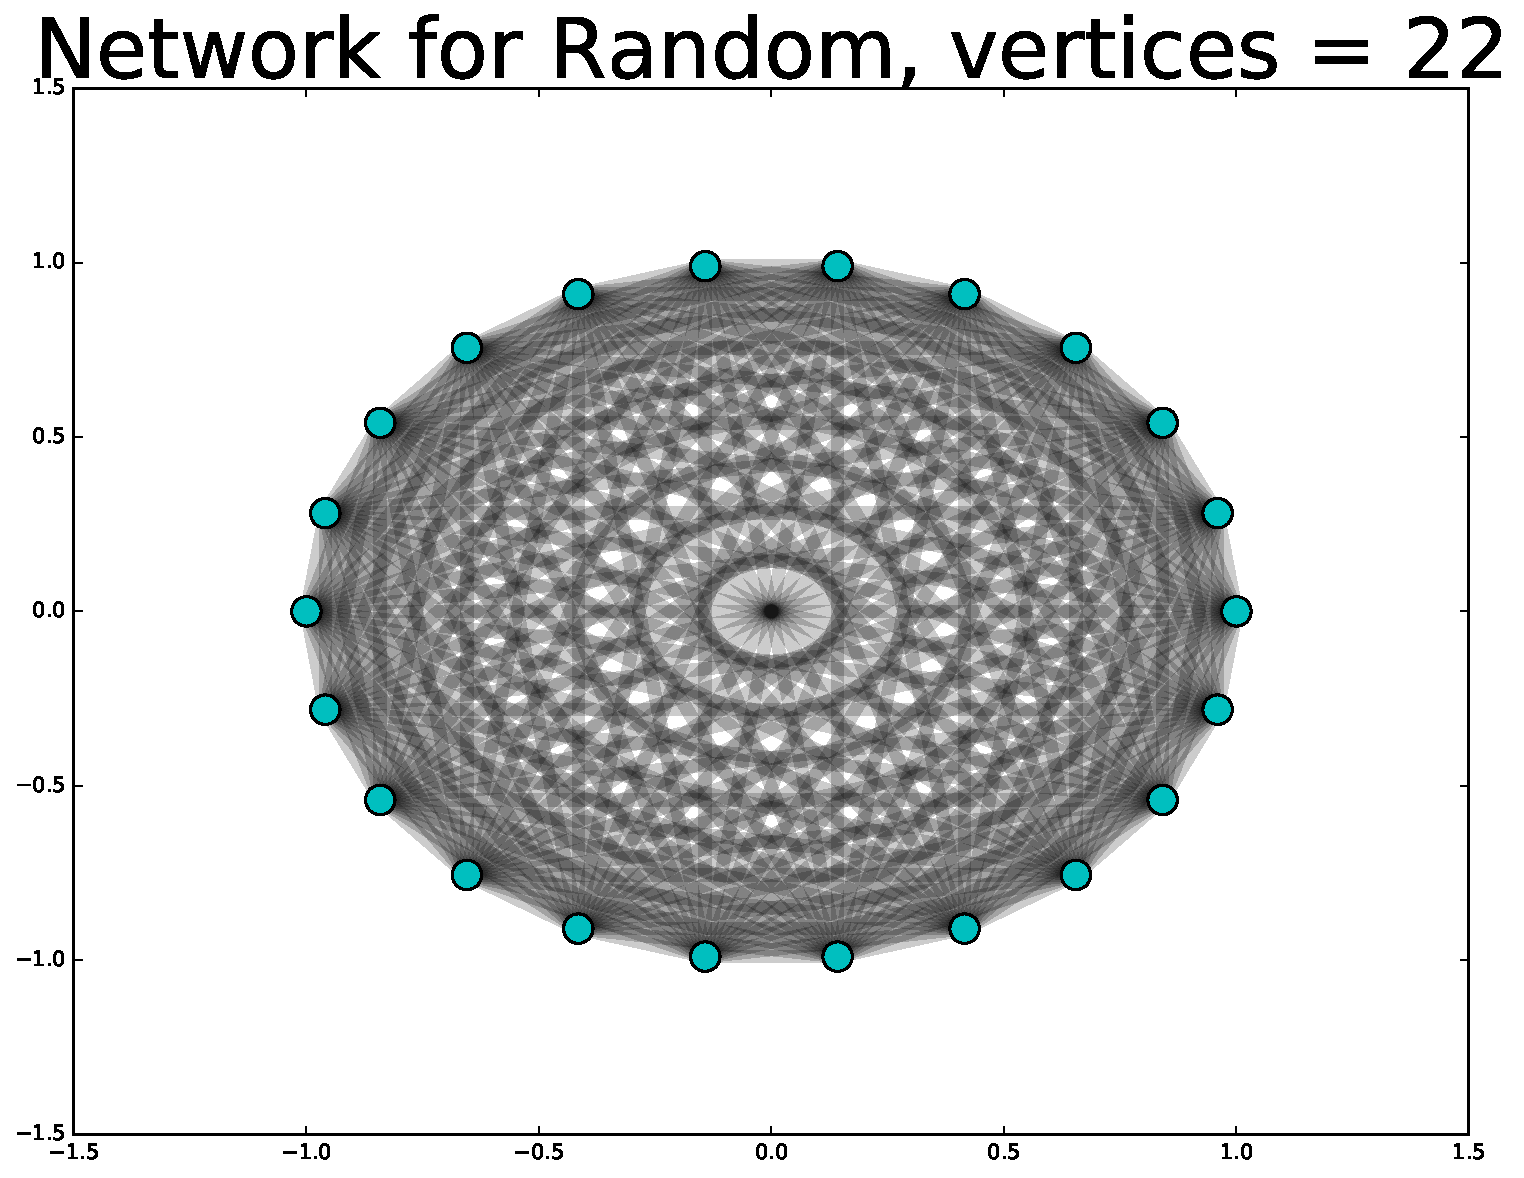
\includegraphics[width=\linewidth]{chapter-four/random_22.pdf}
		\caption{Twenty-two nodes}
	\end{subfigure}
	\caption{Various Erd\"{o}s R\'{e}nyi networks}
	\label{random_networks_illustration}
\end{figure}

To conclude, the complete networks method was the only method where tournament
of 50 players have been played. A total of 500 tournaments, with complete topology,
have been constructed and played through. Table~\ref{table:complete-summary-table}
summarizes, a few of the networks measures. For the complete networks, the measures
could have been predicted, due to the 'all connected rule'. The connectivity
coefficient is equal to the degree. They vary from 1 to 49. One degree value
corresponds to the first network, with a minimum number of nodes 2, and 49 to
the last networks, with a maximum number of 50 nodes.

\begin{table}[!hbtp]
	\centering
	\begin{adjustbox}{width=0.5\textwidth}
		\small
		\begin{tabular}{cccccccccc}
				\toprule
			\multicolumn{5}{|c|}{Complete Networks Summary Table}                     \\ \hline
			     & connectivity & clustering & degree & nodes                  \\ \hline
			mean & 32.70        & 0.99       & 32.70  & 33.70                  \\ \hline
			std  & 11.87        & 0.03       & 11.87  & \multicolumn{1}{c}{-} \\ \hline
			min  & 1.00         & 0.00       & 1.00   & 2.00                   \\ \hline
			max  & 49.00        & 1.00       & 49.00  & 50.00                  \\ \bottomrule
		\end{tabular}
	\end{adjustbox}
	\caption{Complete summary table}
	\label{table:complete-summary-table}
\end{table}

The mean clustering coefficients is set at 0.99 Indicating strong clusters
throughout the experiment, an anticipated result. Furthermore, six random
graphs are displayed in Figure~\ref{complete_networks_illustration}.

\begin{figure}[!hbtp]
	\centering
	\begin{subfigure}[t]{0.30\textwidth}
		\centering
		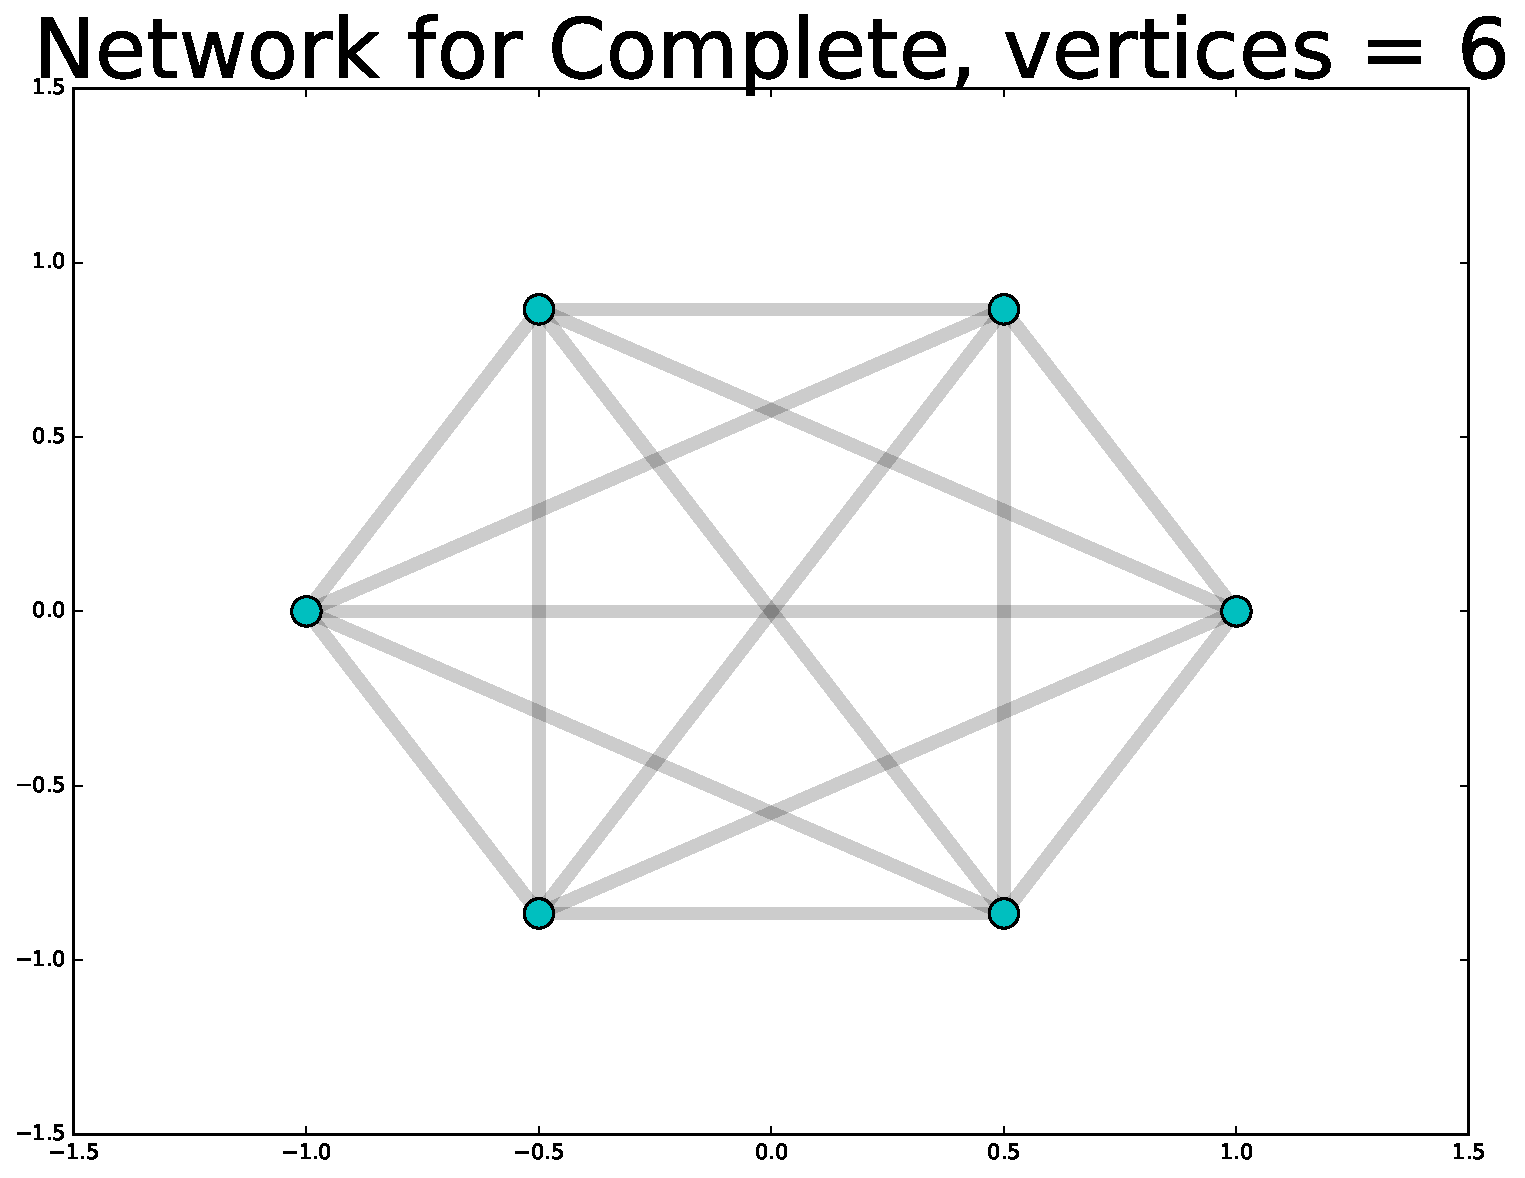
\includegraphics[width=\linewidth]{chapter-four/complete_6.pdf}
		\caption{Six nodes}
	\end{subfigure}
	\hfill
	\begin{subfigure}[t]{0.30\textwidth}\centering
		\centering
		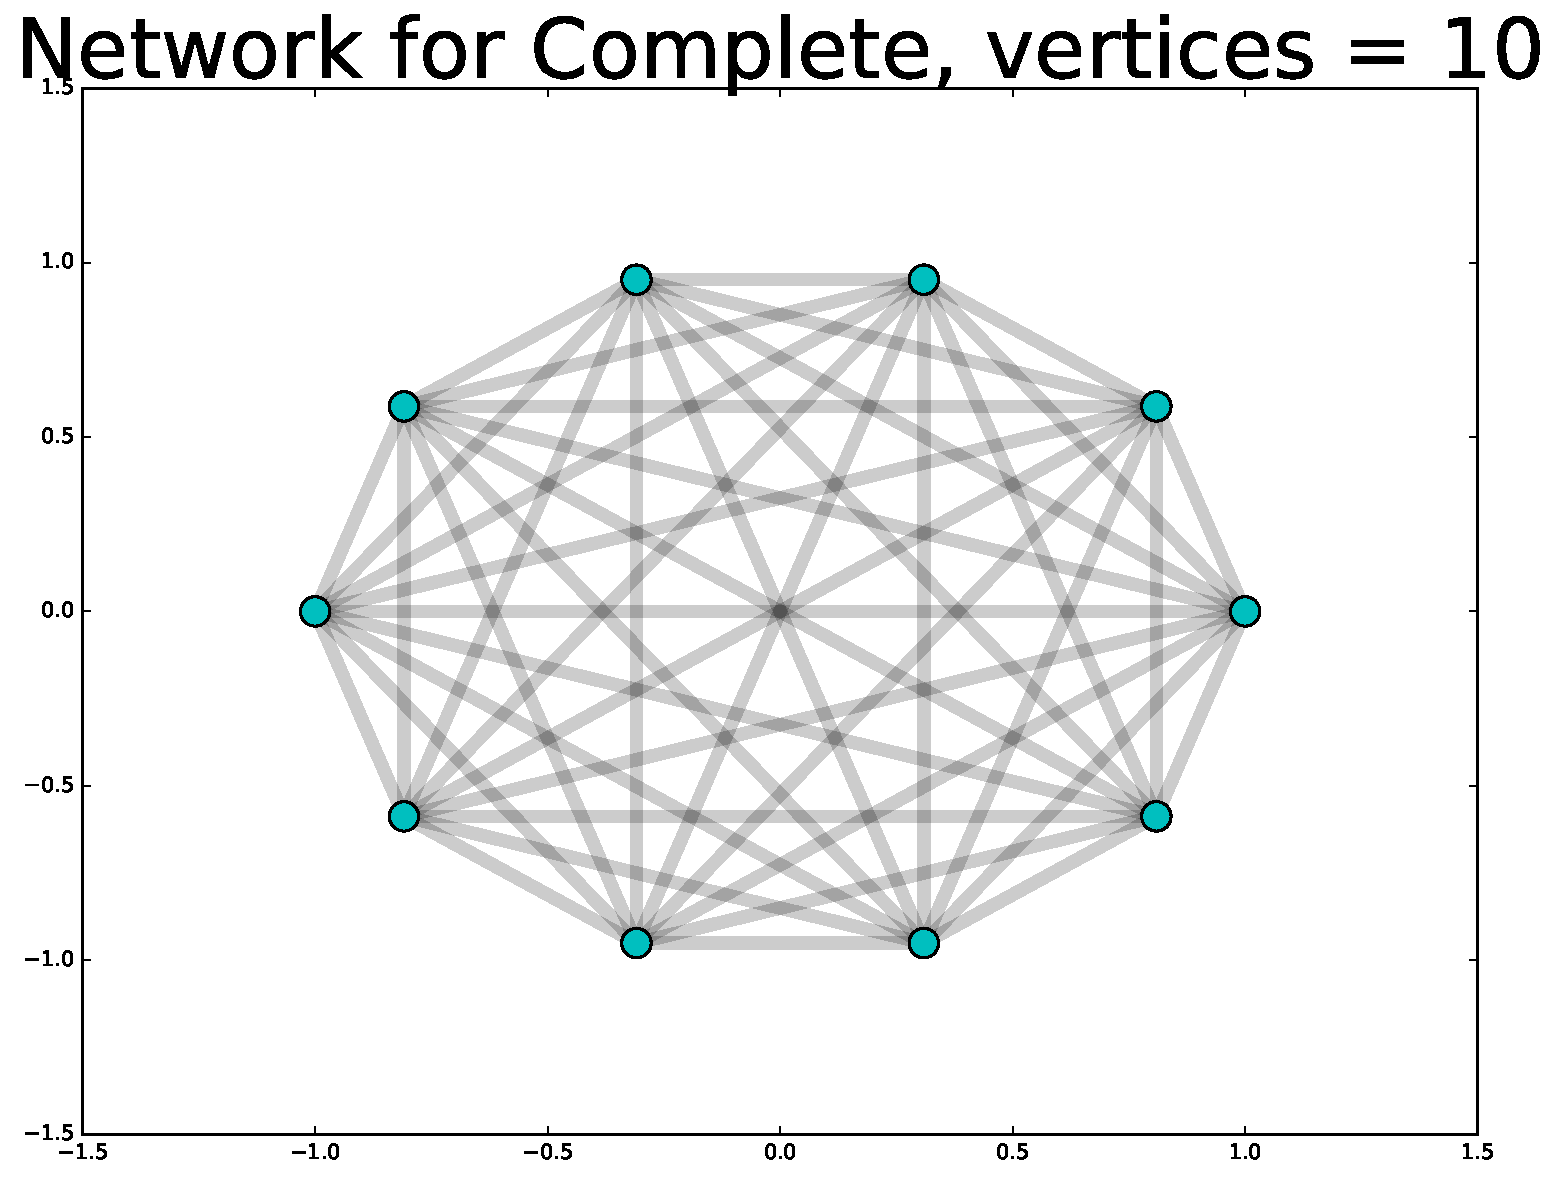
\includegraphics[width=\linewidth]{chapter-four/complete_10.pdf}
		\caption{Ten nodes}
	\end{subfigure}
	\hfill
	\begin{subfigure}[t]{0.30\textwidth}\centering
		\centering
		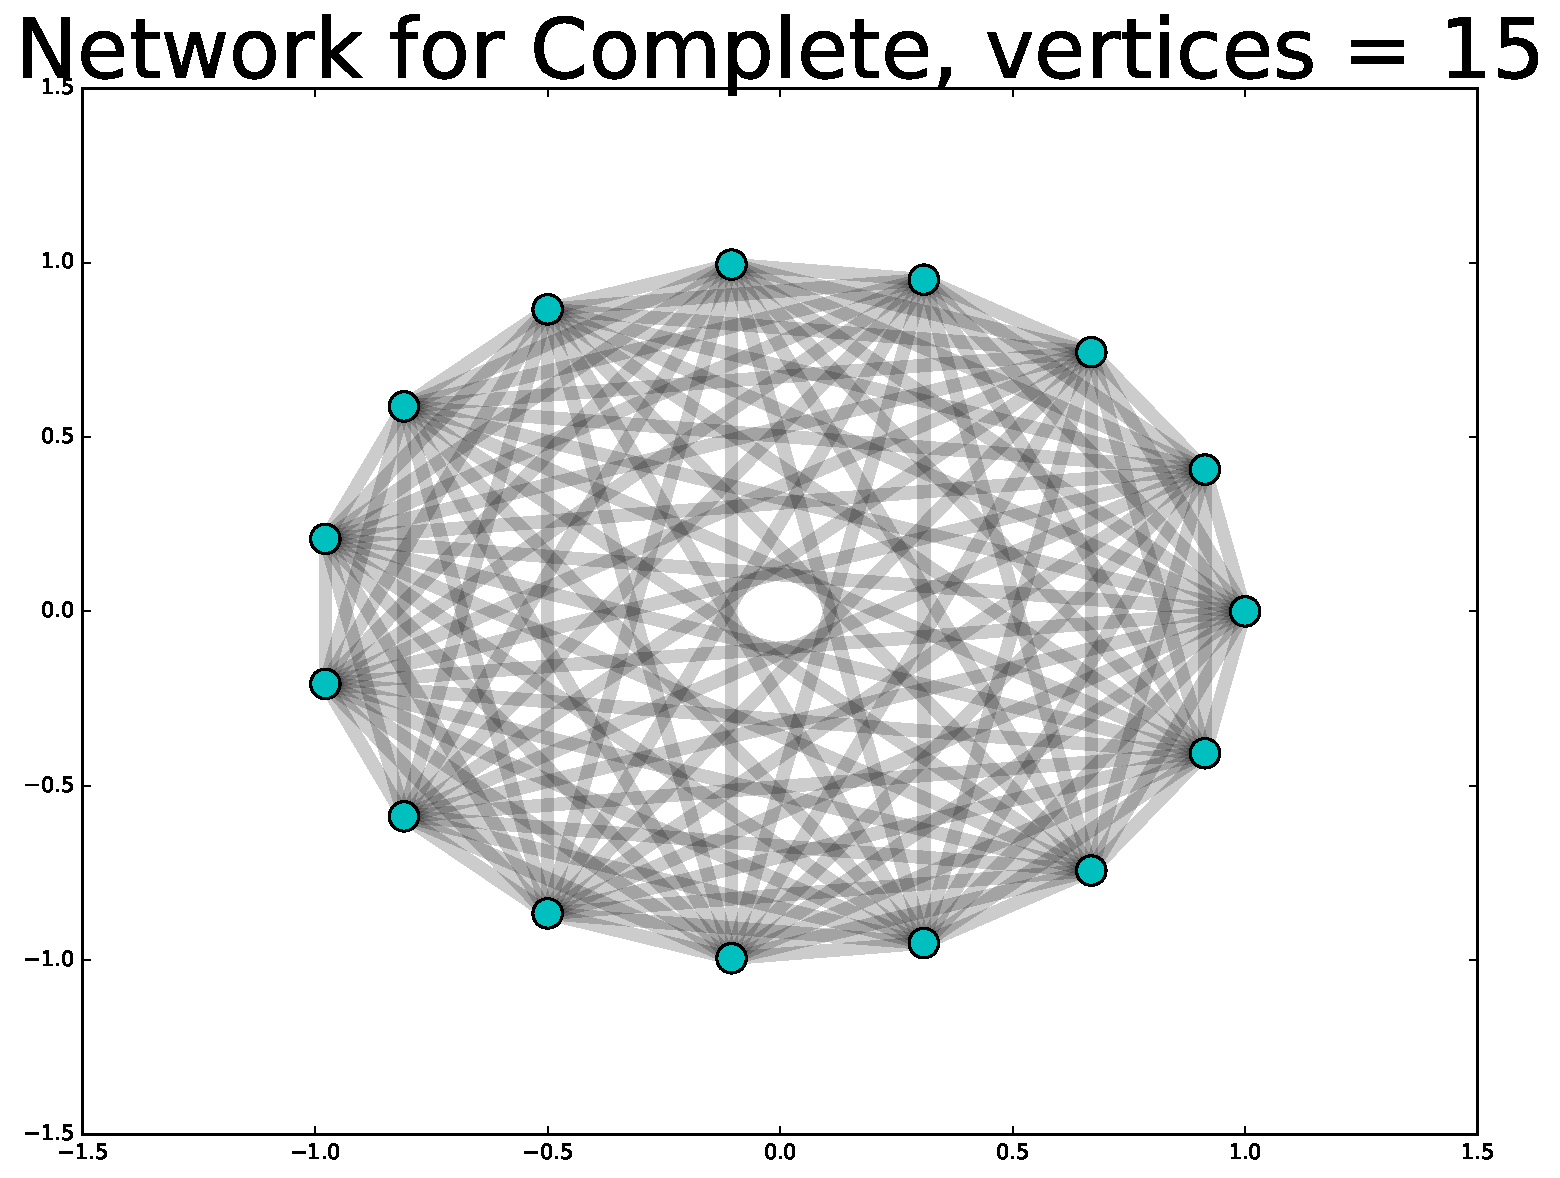
\includegraphics[width=\linewidth]{chapter-four/complete_15.pdf}
		\caption{Fifteen nodes}
	\end{subfigure}
	\hfill
	\begin{subfigure}[t]{0.30\textwidth}\centering
		\centering
		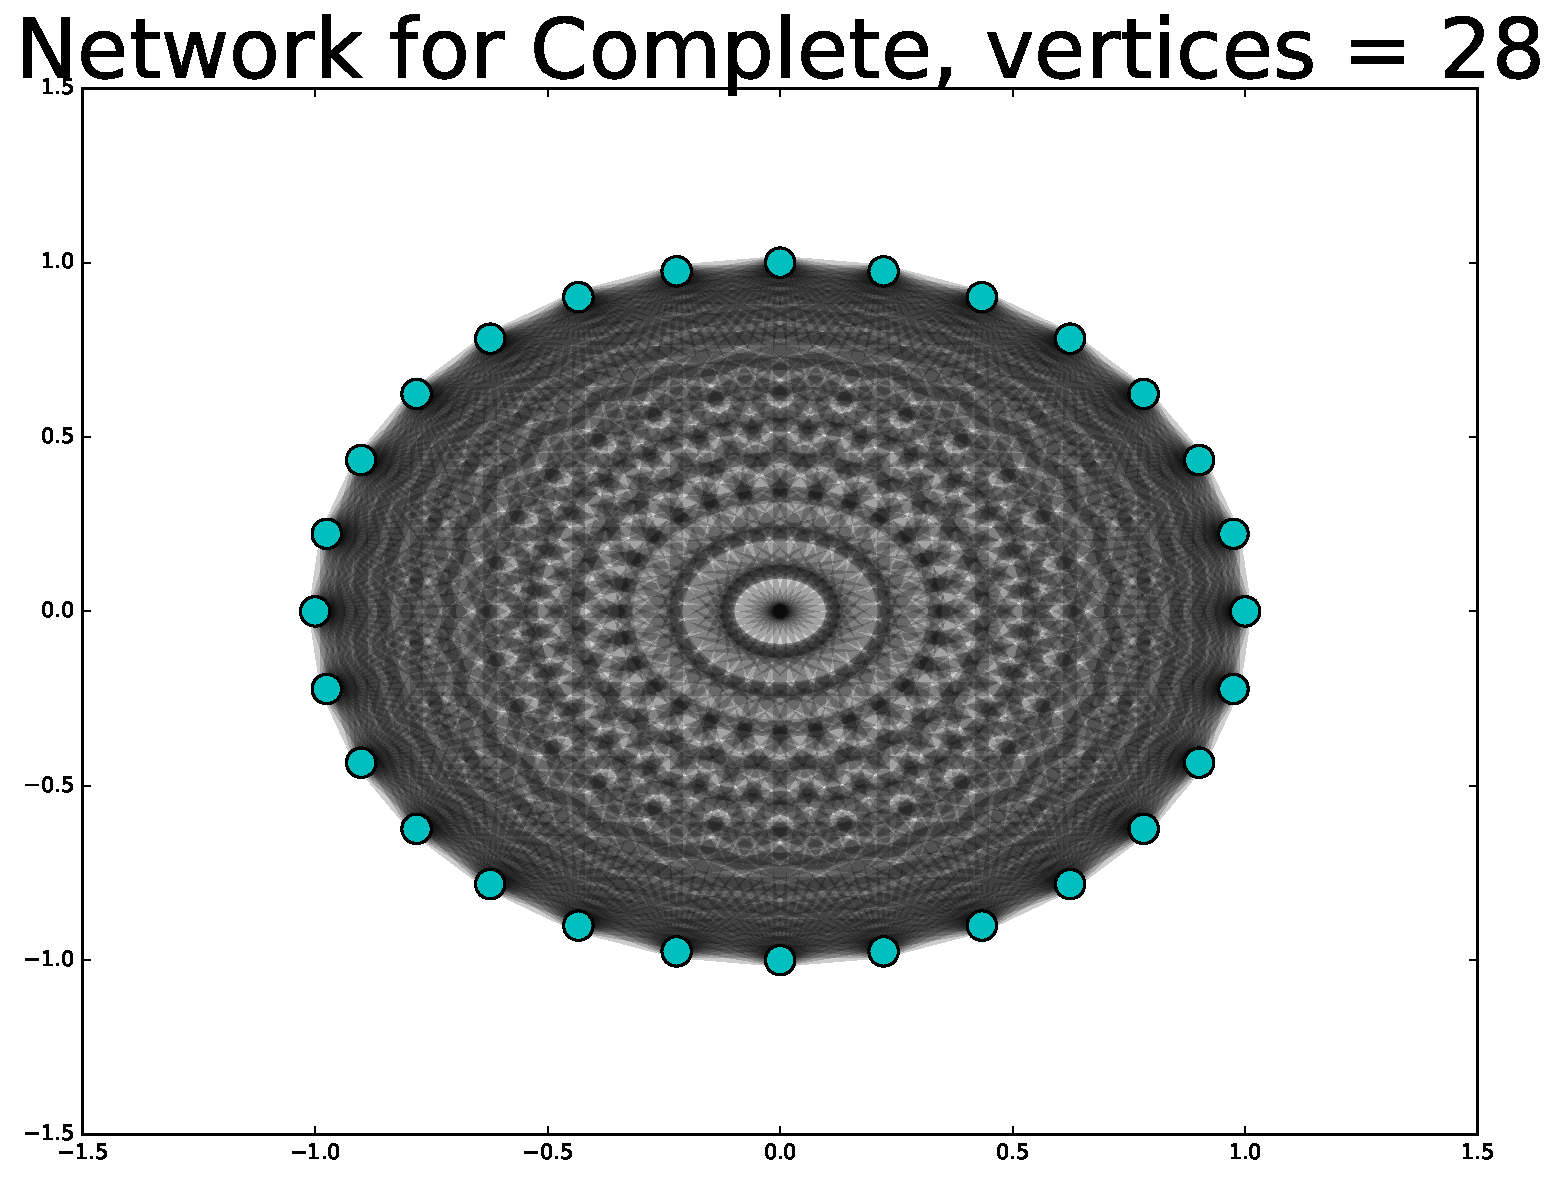
\includegraphics[width=\linewidth]{chapter-four/complete_28.pdf}
		\caption{Twenty-eight nodes}
	\end{subfigure}
	\hfill
	\begin{subfigure}[t]{0.30\textwidth}\centering
		\centering
		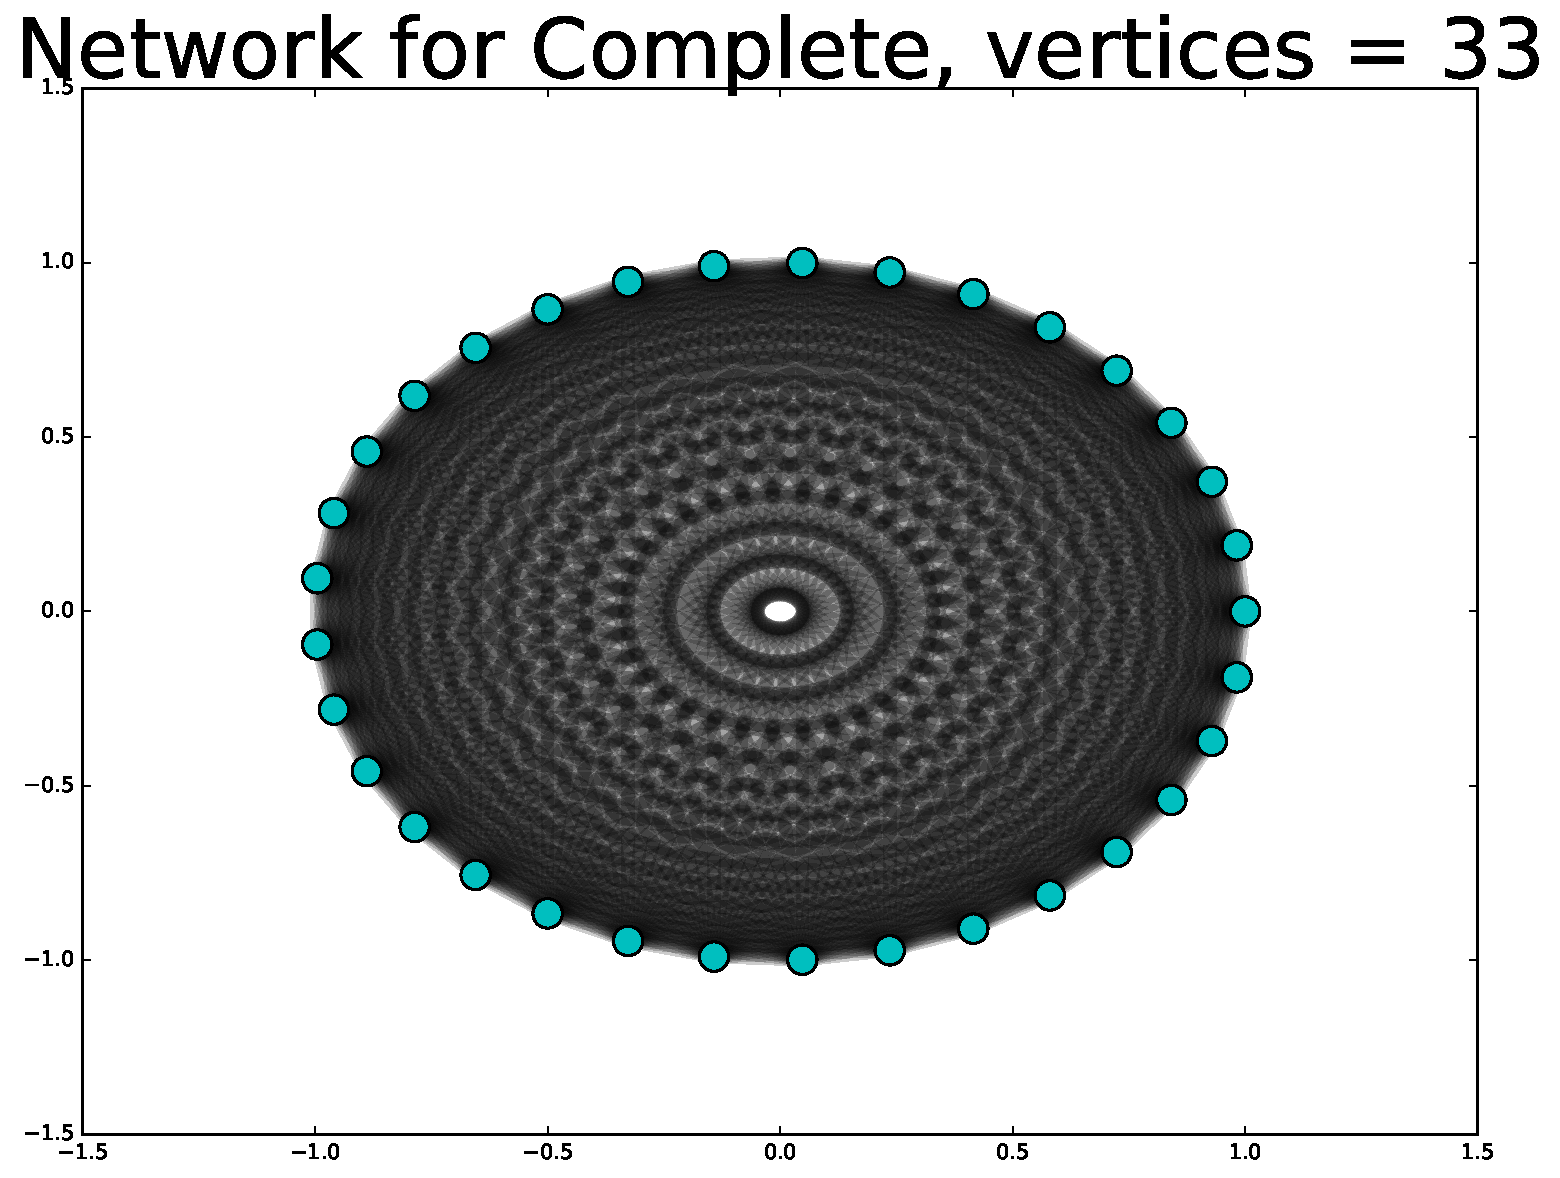
\includegraphics[width=\linewidth]{chapter-four/complete_33.pdf}
		\caption{Thirty-three nodes}
	\end{subfigure}
	\hfill
	\begin{subfigure}[t]{0.30\textwidth}\centering
		\centering
		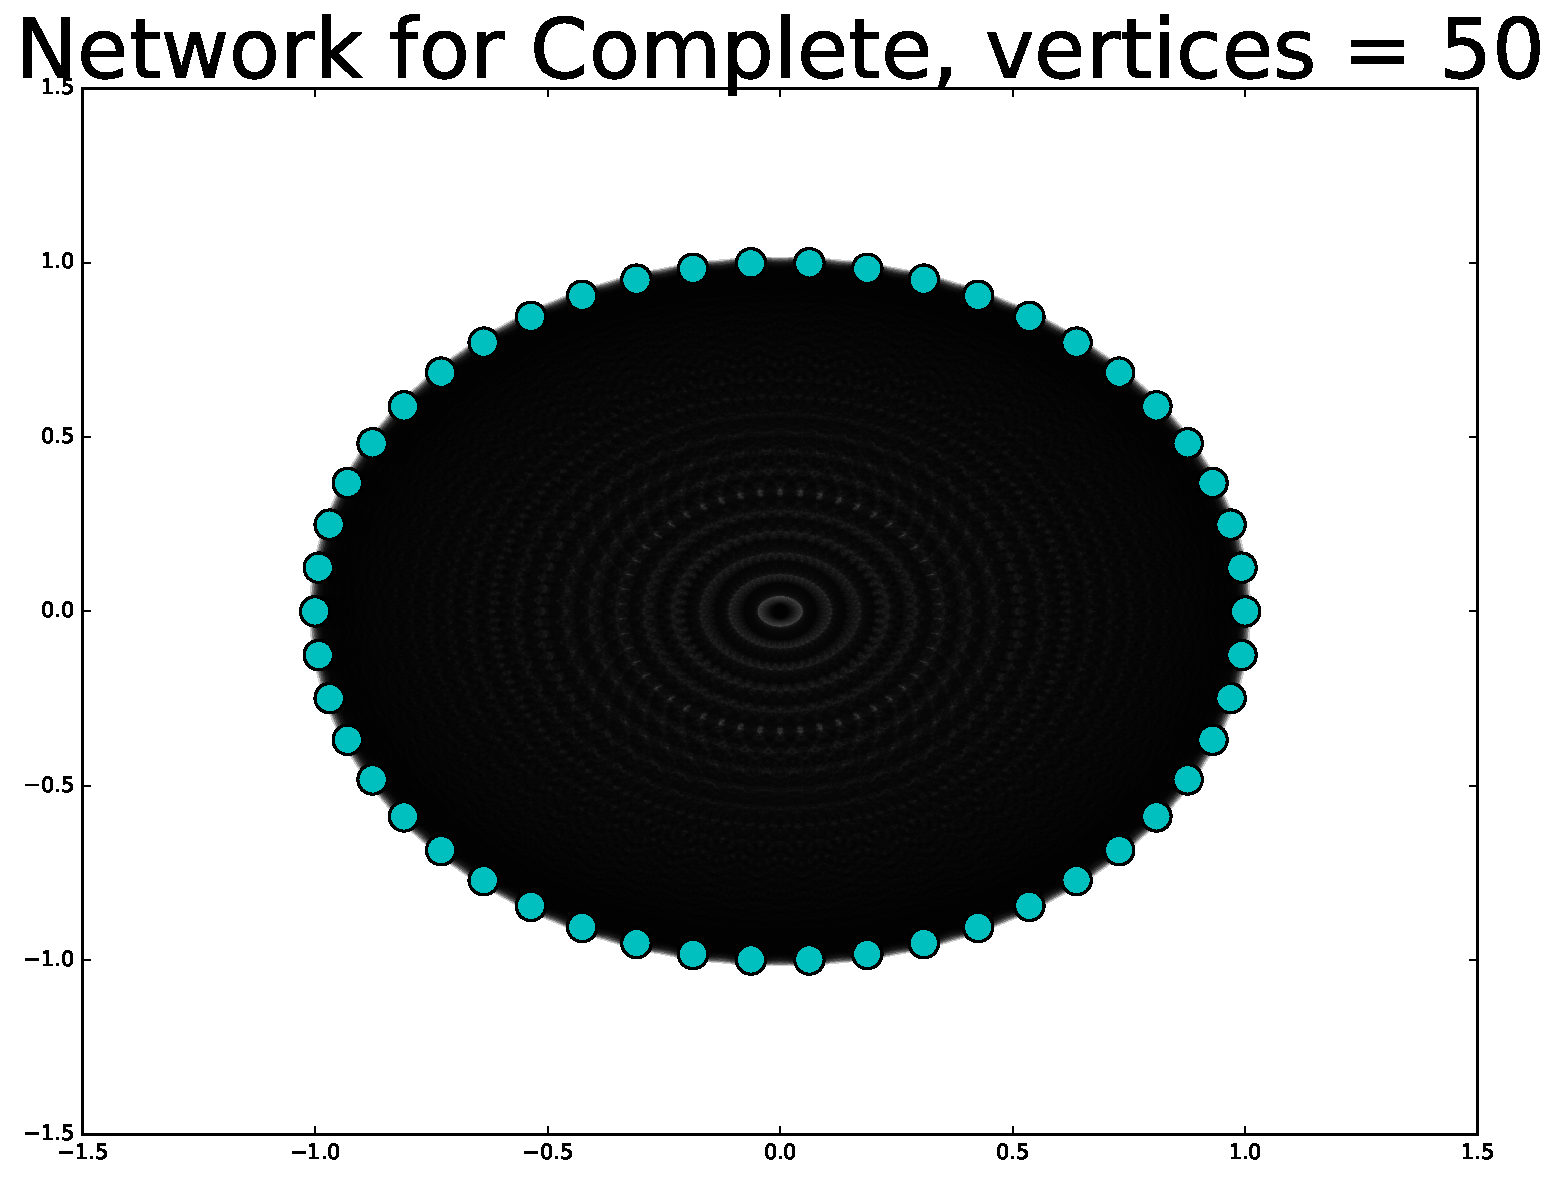
\includegraphics[width=\linewidth]{chapter-four/complete_50.pdf}
		\caption{FIfty nodes}
	\end{subfigure}
	\caption{Various complete networks}
	\label{complete_networks_illustration}
\end{figure}

In this subsection, an initial summary of the overall graphs conducted, in
each of the methods has been held. The number of tournaments, as well as the
tournament size differ. In the following subsection, an initial analysis on the
data produced by each of these methods individually is held.

\subsection{Data Analysis}
This subsection summarizes the results of the tournaments that have been extracted
for the methods.
Individual tables have been managed for each method. The payoff matrix, for
the game of the prisoners dilemmas, follows the payoffs as explained in~\autoref{sub:prisoner-dilemma}.
Thus, punishment payoff is equal to 1 temptation to 5, reward is equal to 3 and
the sucker's payoff is set to 0.

For the small word method the description of the average score, average
neighborhood score, cooperating ratio and neighborhood size are shown in
Table~\ref{table:summary-small-data}. The average score and average
neighborhood score, are fairly equal, both ranging from 0 ($e$, $pi$) to 5 (Fool Me Forever, Bully)
with an average of 2.4. The mean cooperation rating, is equal to 0.64. Thus, strategies behave mostly cooperative.
Mean neighborhood size is 4, which is agreement with~\autoref{sub:network-analysis}.
Maximum neighbors is 9, so even if the maximum players has been 11, no strategy
compete against 10 strategies.

\begin{table}[!hbtp]
	\centering
	\begin{adjustbox}{width=0.8\textwidth}
		\small
		\begin{tabular}{cccccccccc}
				\toprule
			\multicolumn{5}{|c|}{Small world Data Summary Table}                                \\ \hline
			     & average score & average neighborhood & cooperating ratio & neighborhood size \\ \hline
			mean & 2.40          & 2.40                 & 0.64              & 4.74              \\ \hline
			std  & 0.63          & 0.40                 & 0.30              & 2.65              \\ \hline
			min  & 0.00          & 0.00                 & 0.00              & 1.00              \\ \hline
			max  & 5.00          & 5.00                 & 1.00              & 12.00             \\ \bottomrule
		\end{tabular}
	\end{adjustbox}
	\caption{Small world data summary table}
	\label{table:summary-small-data}
\end{table}

For the random method, Table~\ref{summary-random-data} is an initial summary,
for basic measures of the tournaments. Similarly, the average score and average
neighborhood score, are fairly equal. This time, the average neighborhood score,
is slightly lower, 2.38. The minimum average score achieved is 0 ($phi$, $e$, Cycle Hunter)
and the maximum 4.99, again by $e$ and $phi$. Obviously these average scores were achieved in
different tournaments. The mean cooperating ratio, is higher than 0.50.
Thus, strategies tend to cooperate and the neighborhood size, verifies the results
of ~\autoref{sub:network-analysis}.

\begin{table}[!hbtp]
	\centering
	\begin{adjustbox}{width=0.8\textwidth}
		\small
		\begin{tabular}{cccccccccc}
				\toprule
			\multicolumn{5}{|c|}{Random Data Summary Table}                                      \\ \hline
			     & average score & average neighborhood & cooperating ratio & neighborhood size \\ \hline
			mean & 2.38          & 2.38                 & 0.63              & 11.00             \\ \hline
			std  & 0.44          & 0.24                 & 0.25              & 6.57              \\ \hline
			min  & 0.00          & 0.06                 & 0.00              & 1.00              \\ \hline
			max  & 5.00          & 4.99                 & 1.00              & 28.00             \\ \bottomrule
		\end{tabular}
	\end{adjustbox}
	\caption{Random data summary table}
	\label{summary-random-data}
\end{table}

Finally, for the complete experiment, Table ~\ref{table:summary-complete-data}. The
average scores, are lower for this experiment. Both mean average scores are
equal to 2.38. But the maximum average scores, strategies and neighbors, are
below 4. On the other hand, the minimum score are non zero. Specifically,
the minimum average score is equal to 0.55 (Cycler CCD) and the maximum 3.98 (Calculator).
The behavior of the scores can be explained by the topology. In the complete topology experiment,
the highest number of games are played. Considering that for each tournament
\(n-1\) games take place. Thus, scoring zero is less likely because the games
you play are increased by far, and the overall score falls for the same reason.
Cooperating ratio, has a mean value of 0.63 and the neighborhood size
verify what was discussed in ~\autoref{sub:network-analysis}.

\begin{table}[!hbtp]
	\centering
	\begin{adjustbox}{width=0.8\textwidth}
		\small
		\begin{tabular}{cccccccccc}
				\toprule
			\multicolumn{5}{|c|}{Complete Data Summary Table}                                      \\ \hline
			     & average score & average neighborhood & cooperating ratio & neighborhood size \\ \hline
			mean & 2.38          & 2.38                 & 0.63              & 32.70             \\ \hline
			std  & 0.35          & 0.13                 & 0.23              & 11.90             \\ \hline
			min  & 0.55          & 0.54                 & 0.00              & 1.00              \\ \hline
			max  & 3.89          & 3.58                 & 1.00              & 49.00             \\ \bottomrule
		\end{tabular}
	\end{adjustbox}
	\caption{Complete data summary table}
	\label{table:summary-complete-data}
\end{table}

This section has been a preliminary analysis on the outcomes produced by
the three methods. In the upcoming section, more important topics are
raised and an analysis on performance is undertaken.

\section{Performance Analysis}
\label{performance-analysis}
In this section, three measure will be scrutinized, to assess performance of the
strategies. These measures are the winning ratio, the normalized average score
and the median rank. Before hands, the strategies are categorized based on their
average cooperating ratio and the network attributes to which they compete in. Moreover,
various regression models have been constructed for the median rank, and lastly,
the findings are summarized.

\subsection{Classification}
\label{sub:classification}
For being able to conduct the analysis on performance two classifications are
being performed. The two classification that will be conducted are based on:
\begin{itemize}
	\item The average cooperating ratio of the strategies
	\item The networks connectivity and clustering coefficients on the networks
	      used for the spatial tournaments.
\end{itemize}

This is done for the two following reasons. Firstly, as stated in~\autoref{chap:Two},
the Axelrod-Python library (version 1.7.0), consists of 132. Reading though
the documentation for each strategy to distinguish any similarities between
the strategies, would be a challenging task. For this reason, the average cooperation
rating will be used to classify the strategies into categories. Thus, strategies
in the same category will be characterized as similar, based on their level of
cooperation. Secondly, because the performance of the strategies needs to be assessed
based on the topology of the spatial tournament, but networks used itself does
not matter, the clustering and cooperation coefficient are used for a 2 dimensional
clustering.

The clustering will be performed using the popular \(k\)-means algorithm~\cite{kmeans}.
\(k\)-means aims to store observations to k clusters. It stores k centroids
that it used to define cluster. An observation is considered to be in a
particular cluster if it is closer to that cluster's centroid than any other
centroid. The best centroids are identified by:
\begin{itemize}
	\item assigning data points to clusters based on the current centroids
	\item choosing centroids (points which are the center of a cluster) based on
	      the current assignment of data points to clusters.
\end{itemize}

For the average cooperation, five individual categories have been created.
The boundaries of each class and the number of strategies in each category
can been seen in Table~\ref{table:class}, a more detailed table, with the respective category of each
strategy can be found in the Appendix~\ref{append:class-categories}.

Overall six strategies are in the low category. Their average cooperating ratio
ranges between 0.00 and 0.20. In the weak category, the ratio is between
0.23 and 0.40, and is consisted of 17 strategies. 28 strategies are
in the mid category, with upper bound of ratio 0.57 and lower bound a 0.42.
The moderate category, is for strategies which ratio is between 0.58 and 0.75.
Lastly, the high category, with 48 strategies and a mean ratio of 0.87.

\begin{table}[H]
	\centering
	\begin{adjustbox}{width=0.4\textwidth}
		\small
		\begin{tabular}{cccccccccc}
				\toprule
			\multicolumn{5}{|c|}{Classification Table}                        \\ \hline
			Categories & count & \multicolumn{3}{l}{cooperating ratio}        \\ \hline
			         &    & min  & mean & max  \\ \hline
			low      & 6  & 0.00 & 0.10 & 0.20 \\ \hline
			weak     & 17 & 0.23 & 0.32 & 0.40 \\ \hline
			mid      & 28 & 0.42 & 0.50 & 0.57 \\ \hline
			moderate & 33 & 0.58 & 0.65 & 0.75 \\ \hline
			high     & 48 & 0.76 & 0.87 & 1.00 \\ \bottomrule
		\end{tabular}
	\end{adjustbox}
	\caption{Classification table for cooperating ratio}
	\label{table:class}
\end{table}

Applying a 2 dimensional \(k\)-means algorithm to the data, for connectivity and
clustering, returns the following clusters, shown in Table~\ref{table:clusters}.
4 different classes have been created, with means 0.00, 1.00, 2.00 and 3.00 respectively.
In the scatter plot illustrated in Figure~\ref{fig:clusters}, it is clear that only connectivity
affects the means of the clusters. Thus the categories have been named after
the level of connectivity. High connectivity consists of 8100 observations,
moderate connectivity of 75649 observation. Lastly, mid connectivity includes
242405 participants and low connectivity 596259.

\begin{table}[!hbtp]
	\centering
	\begin{adjustbox}{width=0.7\textwidth}
		\small
		\begin{tabular}{cccccccccc}
				\toprule
			\multicolumn{5}{|c|}{Classification Table} \\ \hline
			Categories & number of observation & \multicolumn{3}{l}{connectivity and clustering} \\ \hline
			                      &        & min  & mean & max  \\ \hline
			High connectivity     & 596259 & 0.00 & 0.00 & 0.00 \\ \hline
			Moderate connectivity & 242405 & 1.00 & 1.00 & 1.00 \\ \hline
			Mid connectivity      & 75649  & 2.00 & 2.00 & 2.00 \\ \hline
			Low connectivity      & 8100   & 3.00 & 3.00 & 3.00 \\ \bottomrule
		\end{tabular}
	\end{adjustbox}
	\caption{Classification table for network attributes}
	\label{table:clusters}
\end{table}

\begin{figure}[H]
	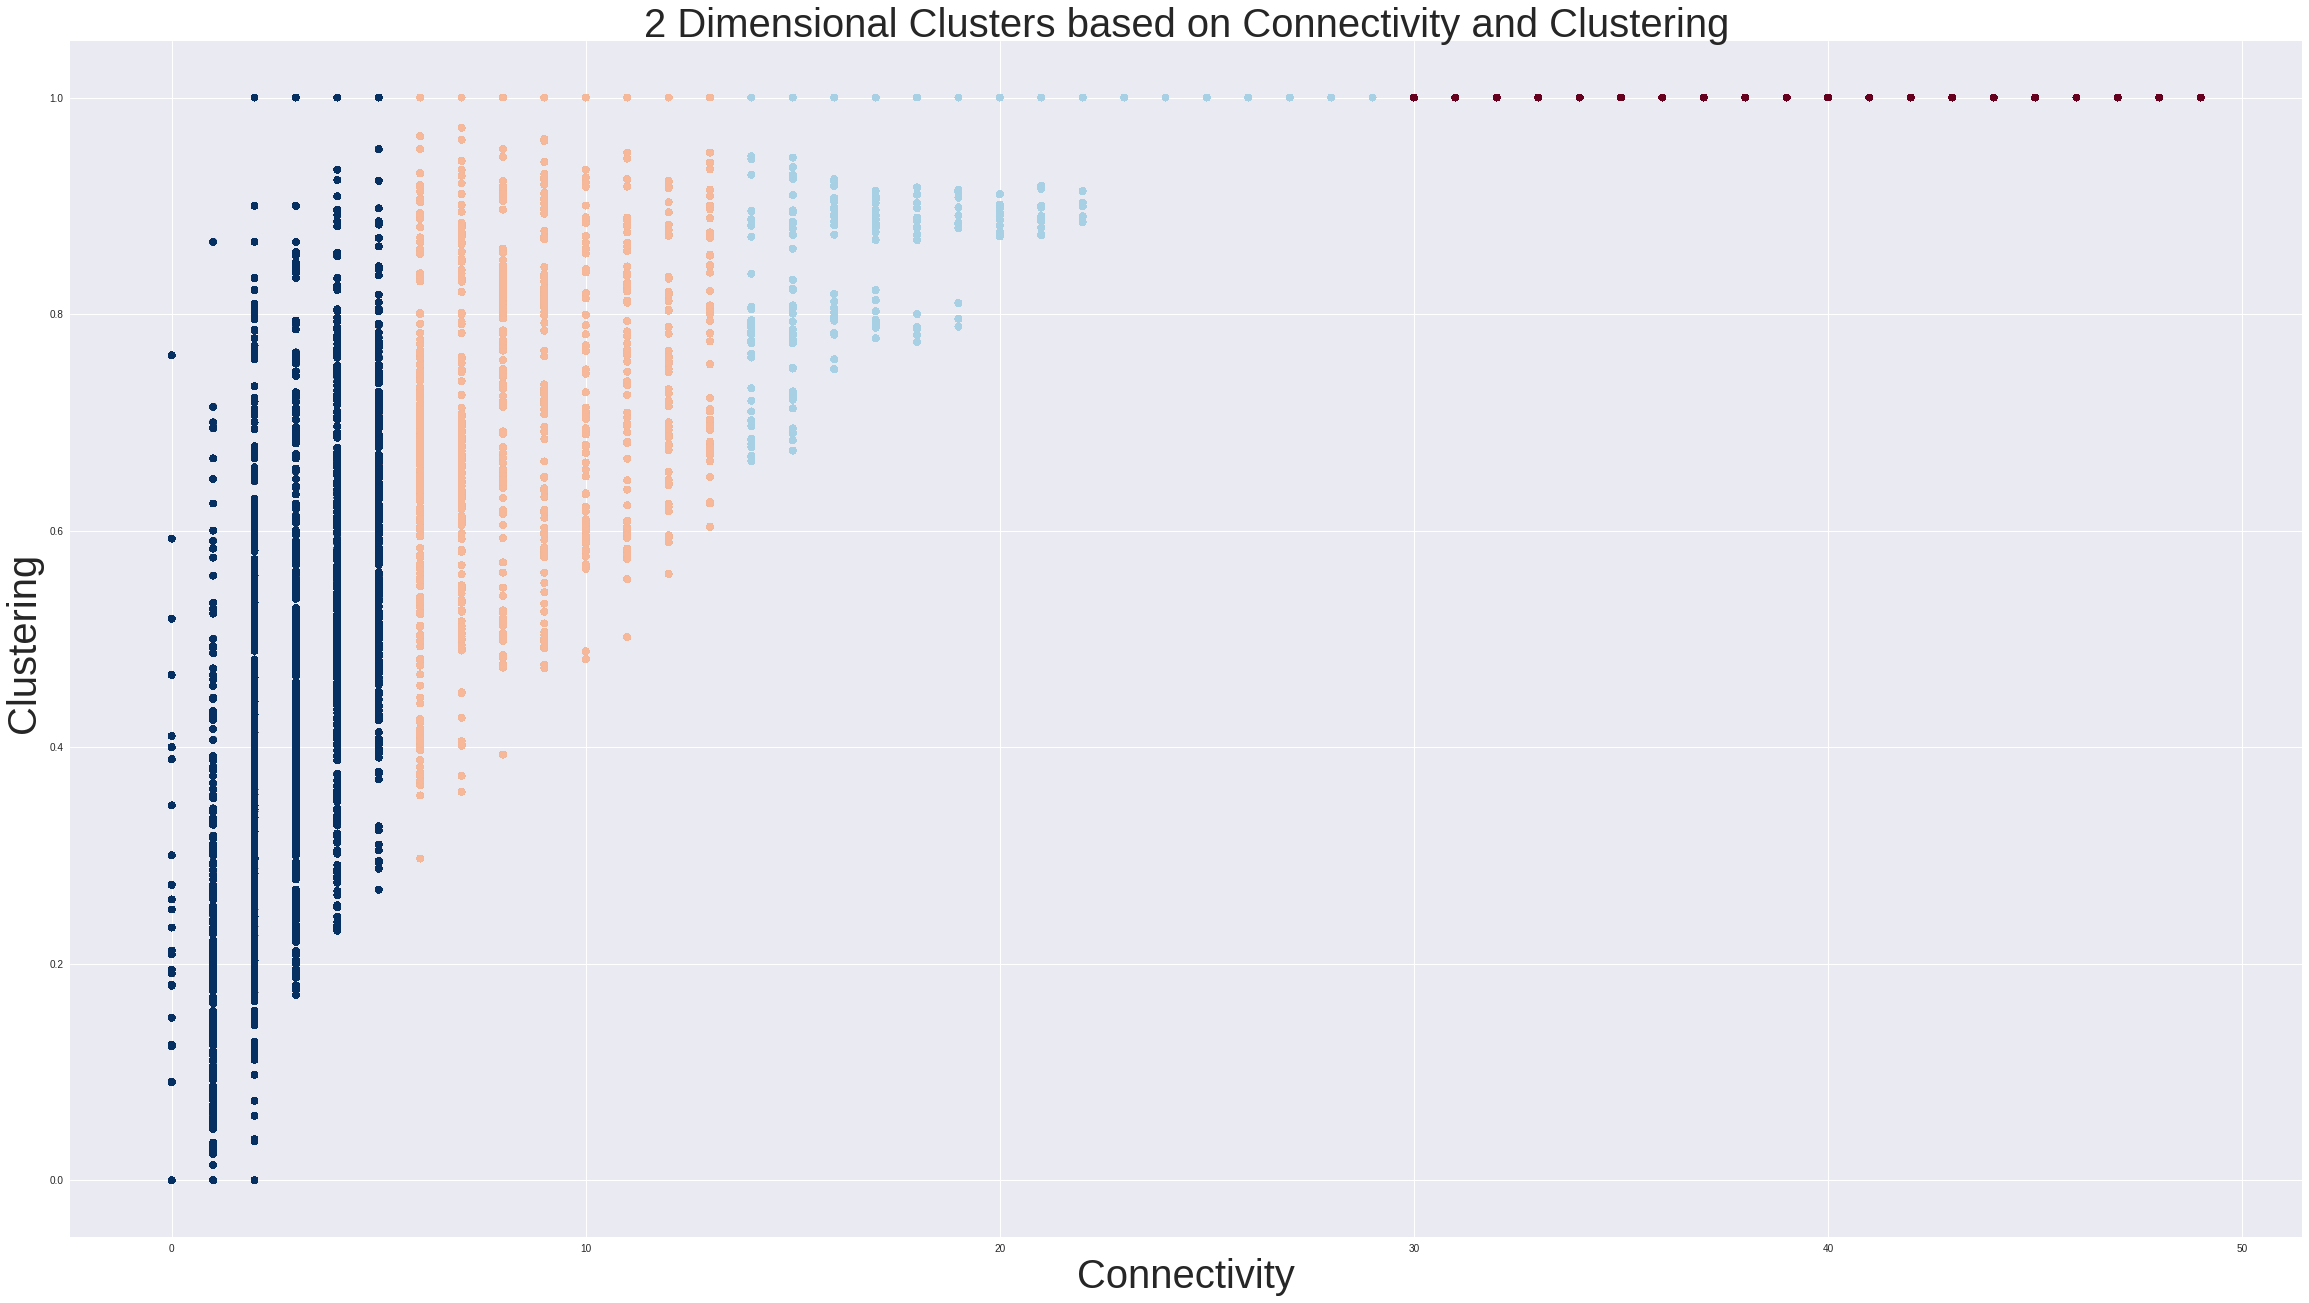
\includegraphics[width=1.2\linewidth,center]{chapter-four/index.png}
	\caption{Clusters based on connectivity and clustering coefficients}
	\label{fig:clusters}
\end{figure}

In this subsection the classification of the strategies and data have been
explained. The classification of the strategies will be a reliable tool
of similarity in the following subsections, and now that the network
attributes have been clusters they will be used further in the analysis.

\subsection{Winning Ratio}
In this subsection, the strategies are being assessed based on the winning ratio.
The strategies have been ranked, and Figure~\ref{fig:wining-second-gen}
illustrates the strategies with ascending order. The highest ranked strategies,
are:
\begin{itemize}
	\item Fool Me Forever, a high cooperative strategy, with a winning ratio of 0.178
	\item Grumpy, a high cooperative strategy, with a winning ratio of 0.179
	\item Ripoff, a mid cooperative strategy, with a winning ratio of 0.187
	\item Cycler DDC, a weak cooperative strategy, with a winning ratio of 0.203
	\item Calculator, a weak cooperative strategy, with a winning ratio of 0.228
\end{itemize}

Even though, Fool Me Forever, Grumpy, are characterized as highly
cooperatives strategies, Cycler DDC and Calculator are weak cooperators. The
strategies that have achieved zero wining ratio are listed here:
\begin{itemize}
	\item Fortress4, a low cooperative strategy
	\item Math Constant Hunter, a moderate cooperative strategy
	\item Win-Shift Lose-Stay, a mid cooperative strategy
	\item Once Bitten, a high cooperative strategy
	\item ThueMorseInverse, a mid cooperative strategy
	\item Retaliate (0.1), a moderate cooperative strategy
\end{itemize}

\begin{figure}[H]
	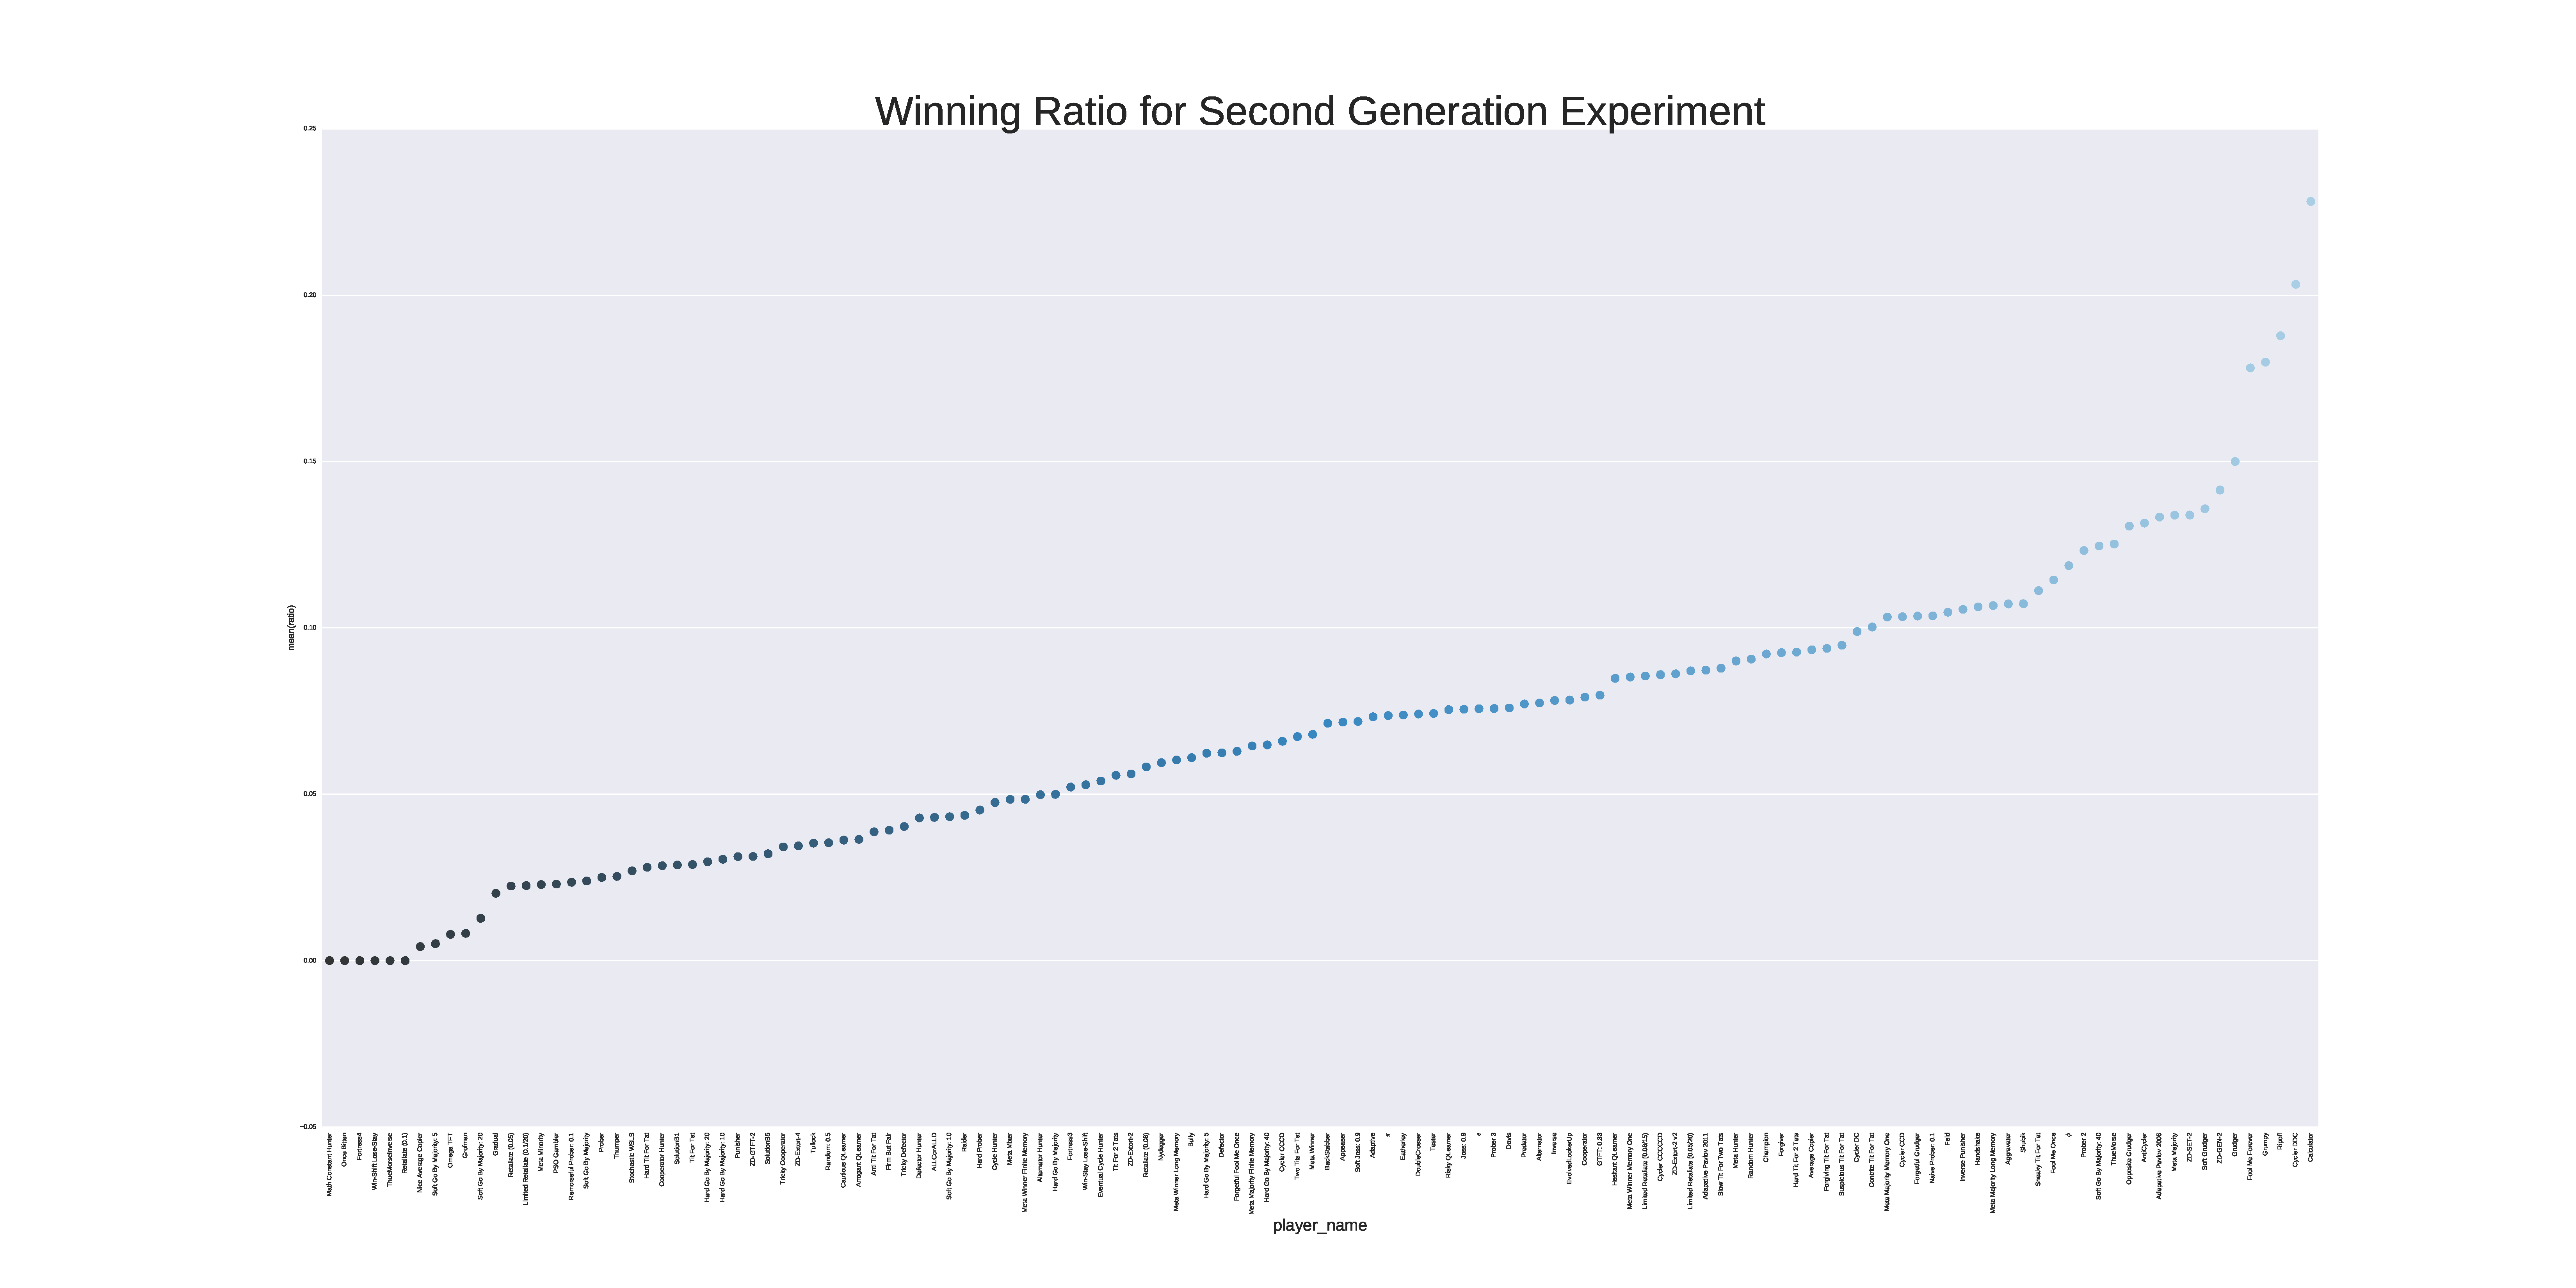
\includegraphics[width=1.2\linewidth,center]{chapter-four/winning-ratio.pdf}
	\caption{Ranks based on winning ratio}
	\label{fig:wining-second-gen}
\end{figure}

There seems to be no correlation between that winning ratio and the cooperation
categories. Furthermore, due the conclusion of ~\autoref{chap:Three}, winning ratio was described as
an non fitting performance measure. Thus, no more attention will be given to
winning ratio. In the following subsections, there is a briefly discussion of the
normalized average score and afterwards an in depth analysis on the normalized
ranking.

\subsection{Normalized Average Score}
\label{sub:chap-four-normalized-score}
In this subsection, the normalized average score is studied. The strategies
have been ranked based on their mean normalized score, and Figure~\ref{fig:wining-second-gen} illustrates
the ranks with ascending order. The highest ranked strategies have been:

\begin{itemize}
	\item PSO Gambler, a moderate cooperative strategy, with a mean score of 0.005386
	\item Win-Shift Lose-Stay, a mid cooperative strategy, with a mean score of 0.052707
	\item Prober, a weak cooperative strategy, with a mean score of 0.055400
	\item Retaliate (0.1), a moderate cooperative strategy, with a mean score of 0.121850
	\item Once Bitten, a high cooperative strategy, with a mean score of 0.290005
	\item Fortress4, a high cooperative strategy, with a mean score of 0.413419
\end{itemize}

As shown in Figure~\ref{fig:wining-second-gen}, there is a massive gap between
the top 5 strategies and the rest, based on normalized score. On the other hand
the lowest ranked strategies were:

\begin{itemize}
	\item $e$, a high cooperative strategy, with a mean score of 0.000085
	\item Joss: 0.9, a mid cooperative strategy, with a mean score of 0.000098
	\item Suspicious Tit For Tat, a mid cooperative strategy, with a mean score of 0.000105
	\item Handshake, a low cooperative strategy, with a mean score of 0.000114
	\item Opposite Grudger, a high cooperative strategy, with a mean score of 0.000119
\end{itemize}

The highest ranked strategies of the mean score differ from the strategies that
have hab the highets rank based on wining ratio. In addition, as was also seen
in ~\autoref{chap:Three}, a highest rank strategy based on the normalized score,
Fortress4, has been ranked as a low performance strategy based on the winning ratio.
Thus, there is a conflict created in the results. For this reason, normalized
average score will not be investigated further, on the next subsection normalized
rank is being introduced.

\begin{figure}[H]
	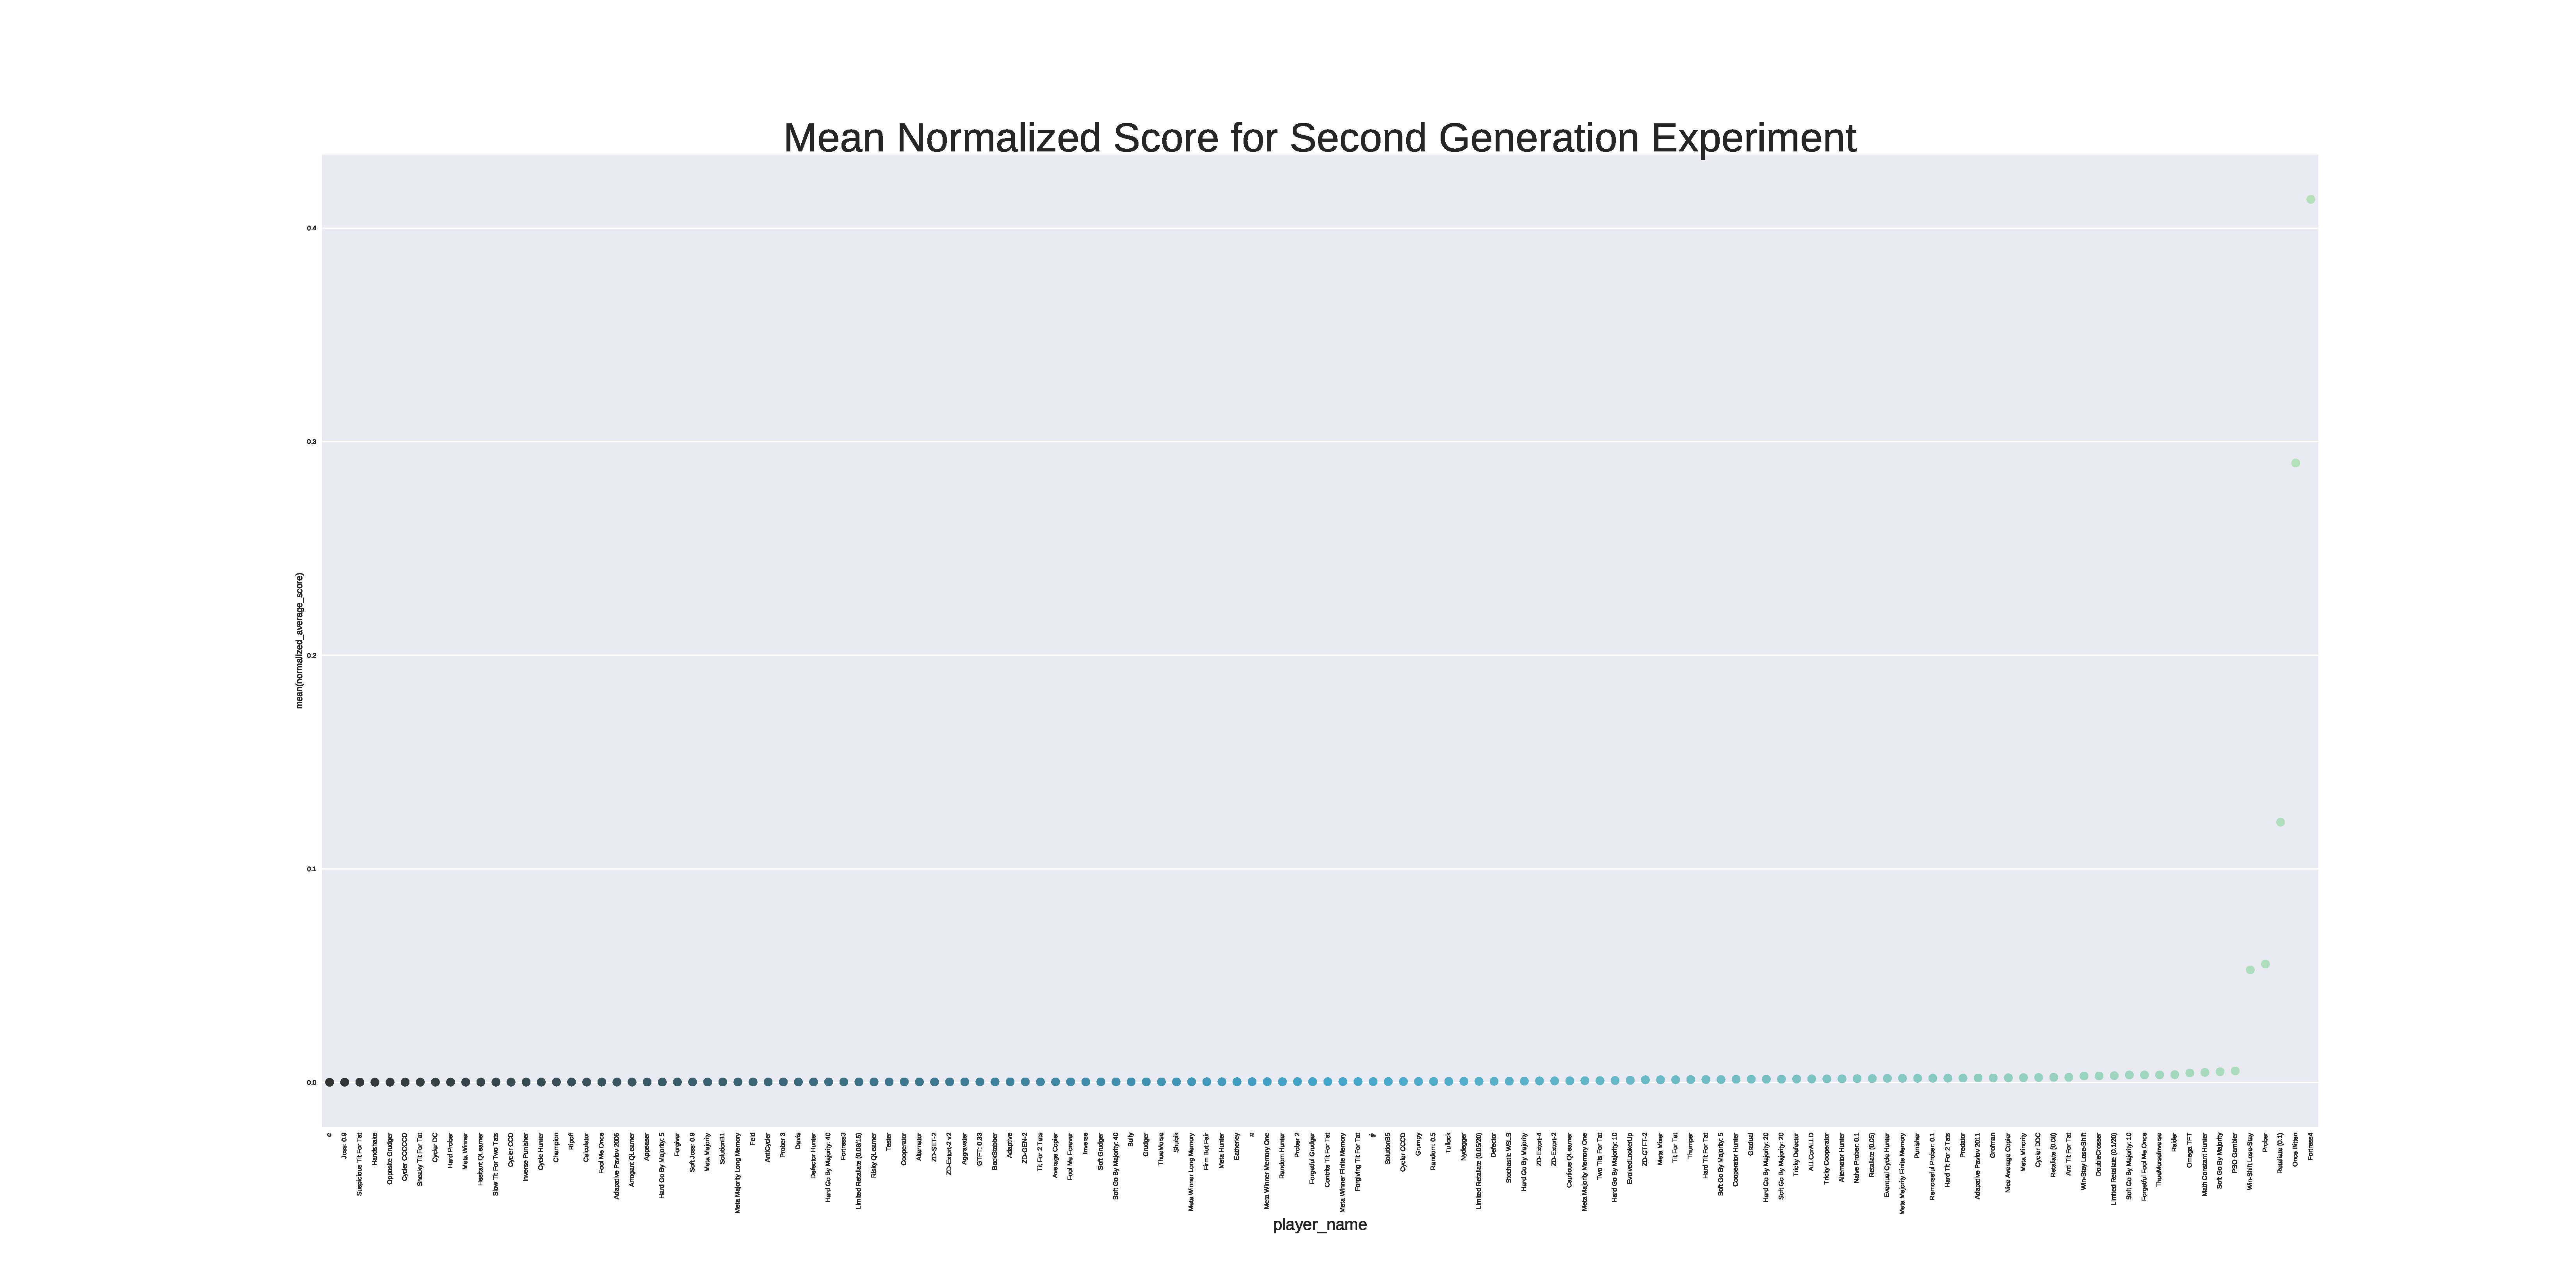
\includegraphics[width=1.2\linewidth,center]{chapter-four/score-ranking.pdf}
	\caption{Ranks based on normalized score}
	\label{fig:wining-second-gen}
\end{figure}

\subsection{Median Normalized Rank}

This part of the chapter, focuses on a new measure of performance. The
median normalized rank of the strategies. The normalized rank is computed
by dividing each rank of a strategy for a specific tournament by the corresponding
size of the tournament. The median rank is believed to be a more accurate
measure of performance, compared to winning ratio and normalized score.
As it will reveal strategies, that did not necessarily achieved the maximum wins,
but had an overall satisfying and smoothly performance throughout the experiment.

The median normalized score has been computed for each strategy and the ranks
are illustrated by the point plot in Figure~\ref{fig:ranking-second-gen}.~\footnote{A reminder,the
	lowest the rank the higher a strategy scored. 0 is the highest rank a strategy
can achieve in a tournament.} The strategies with the lowest median ranking are,
Meta Majority Finite Memory, Meta Minority and Limited Retaliate (0.1/20).
On the other hand, the highest ranked strategies are the following:

\begin{itemize}
	\item Fourth with a median ranking equal to 0.29, PSO Gambler
	\item Third with a median ranking equal to 0.27, Nydegger
	\item Second with a median ranking equal to 0.25, Cautious QLearner
	\item First with a median ranking equal to 0.23, Gradual
\end{itemize}

\begin{figure}[!hbtp]
	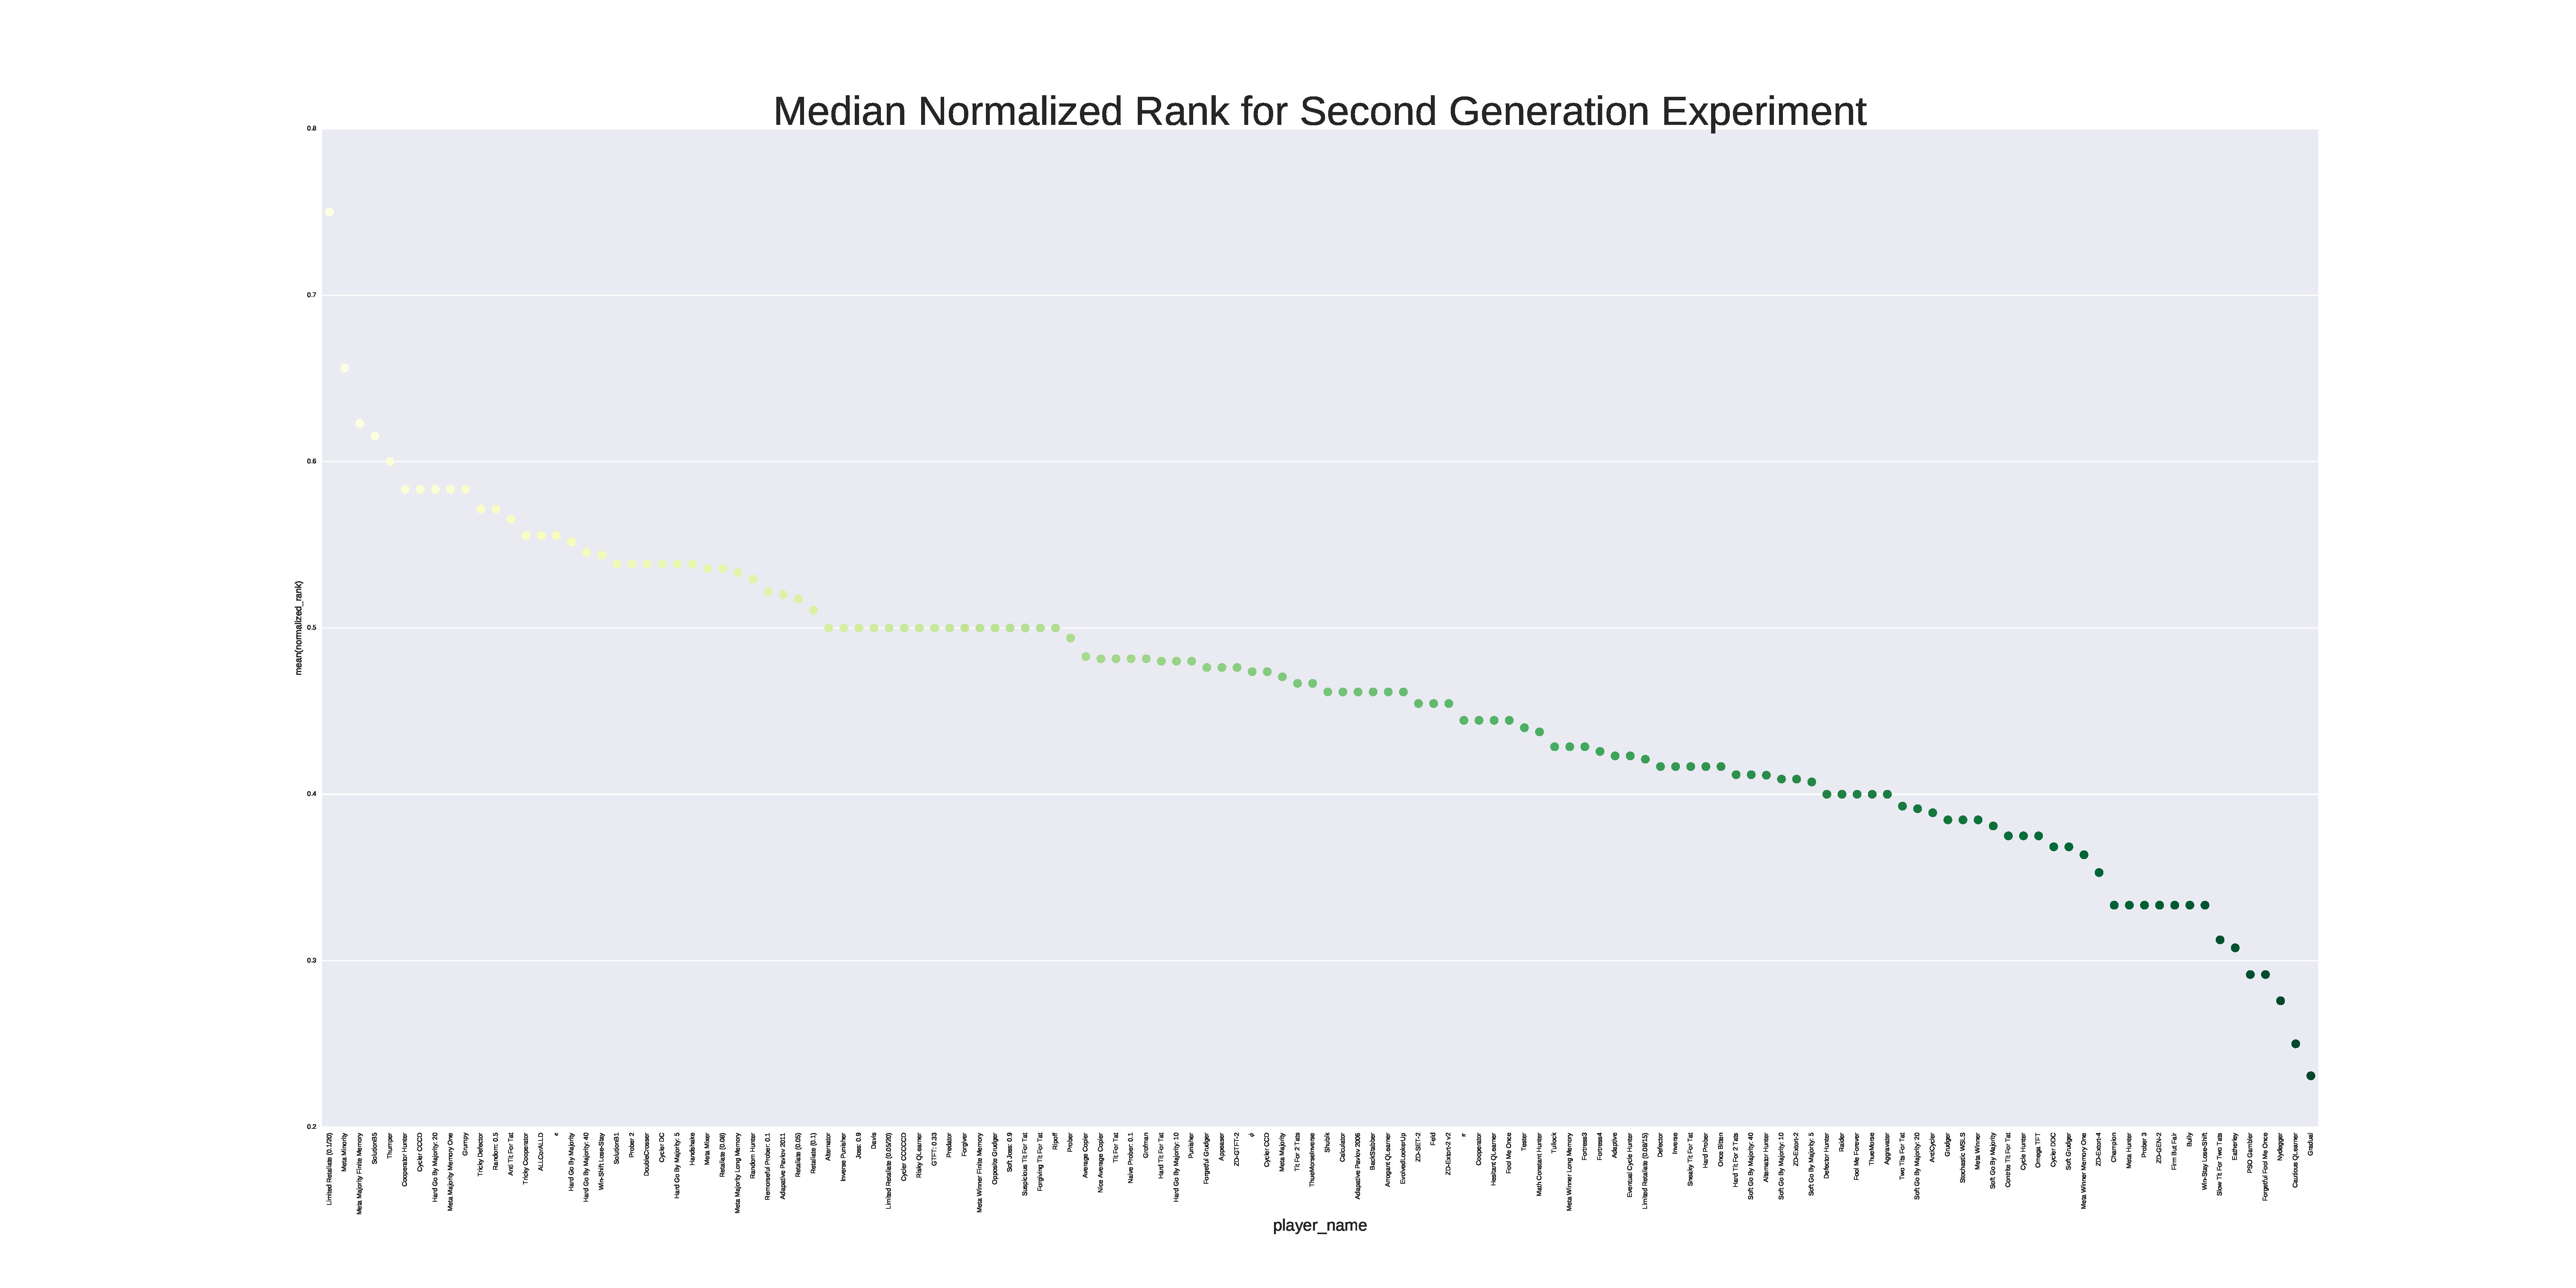
\includegraphics[width=1.2\linewidth,center]{chapter-four/median-ranking.pdf}
	\caption{Normalized median rank for complex networks experiments}
	\label{fig:ranking-second-gen}
\end{figure}

Both PSO Gambler and Gradual are well performed strategies in the Axlerod-Python
tournament. Furthermore, apart from PSO Gamber, which is a moderate cooperative
strategy, the rest are characterized as high cooperators. Further research on
the cooperation ratio will be executed in the following subsection.

To investigate the effect of networks topologies in the findings, a Kruskal Wallis test
has been executed. The existence of a statistically significant difference between
the normalized ranking and the clustered groups, as stated in ~\autoref{sub:classification} based on the
connectivity and clustering coefficients, is being tested. A non parametric test
is used, because ranks are not a normally distributed measure. For the Kruskal Wallis
test the \texttt{scipy} Python library is being used once again.

The finding of the tests returned the following results. There is significant
difference on the normalized ranking between the clustered groups (\(p\)
value less than 0.05). Thus, depending on the topology the ranks differ.
Figure~\ref{fig:variation-clusters}, shows that there is a increasing trend.
Because the clusters seems to be affected more from the connectivity coefficients,
it could be assumed that as the connectivity increases the rank does as well.

\begin{figure}[!hbtp]
	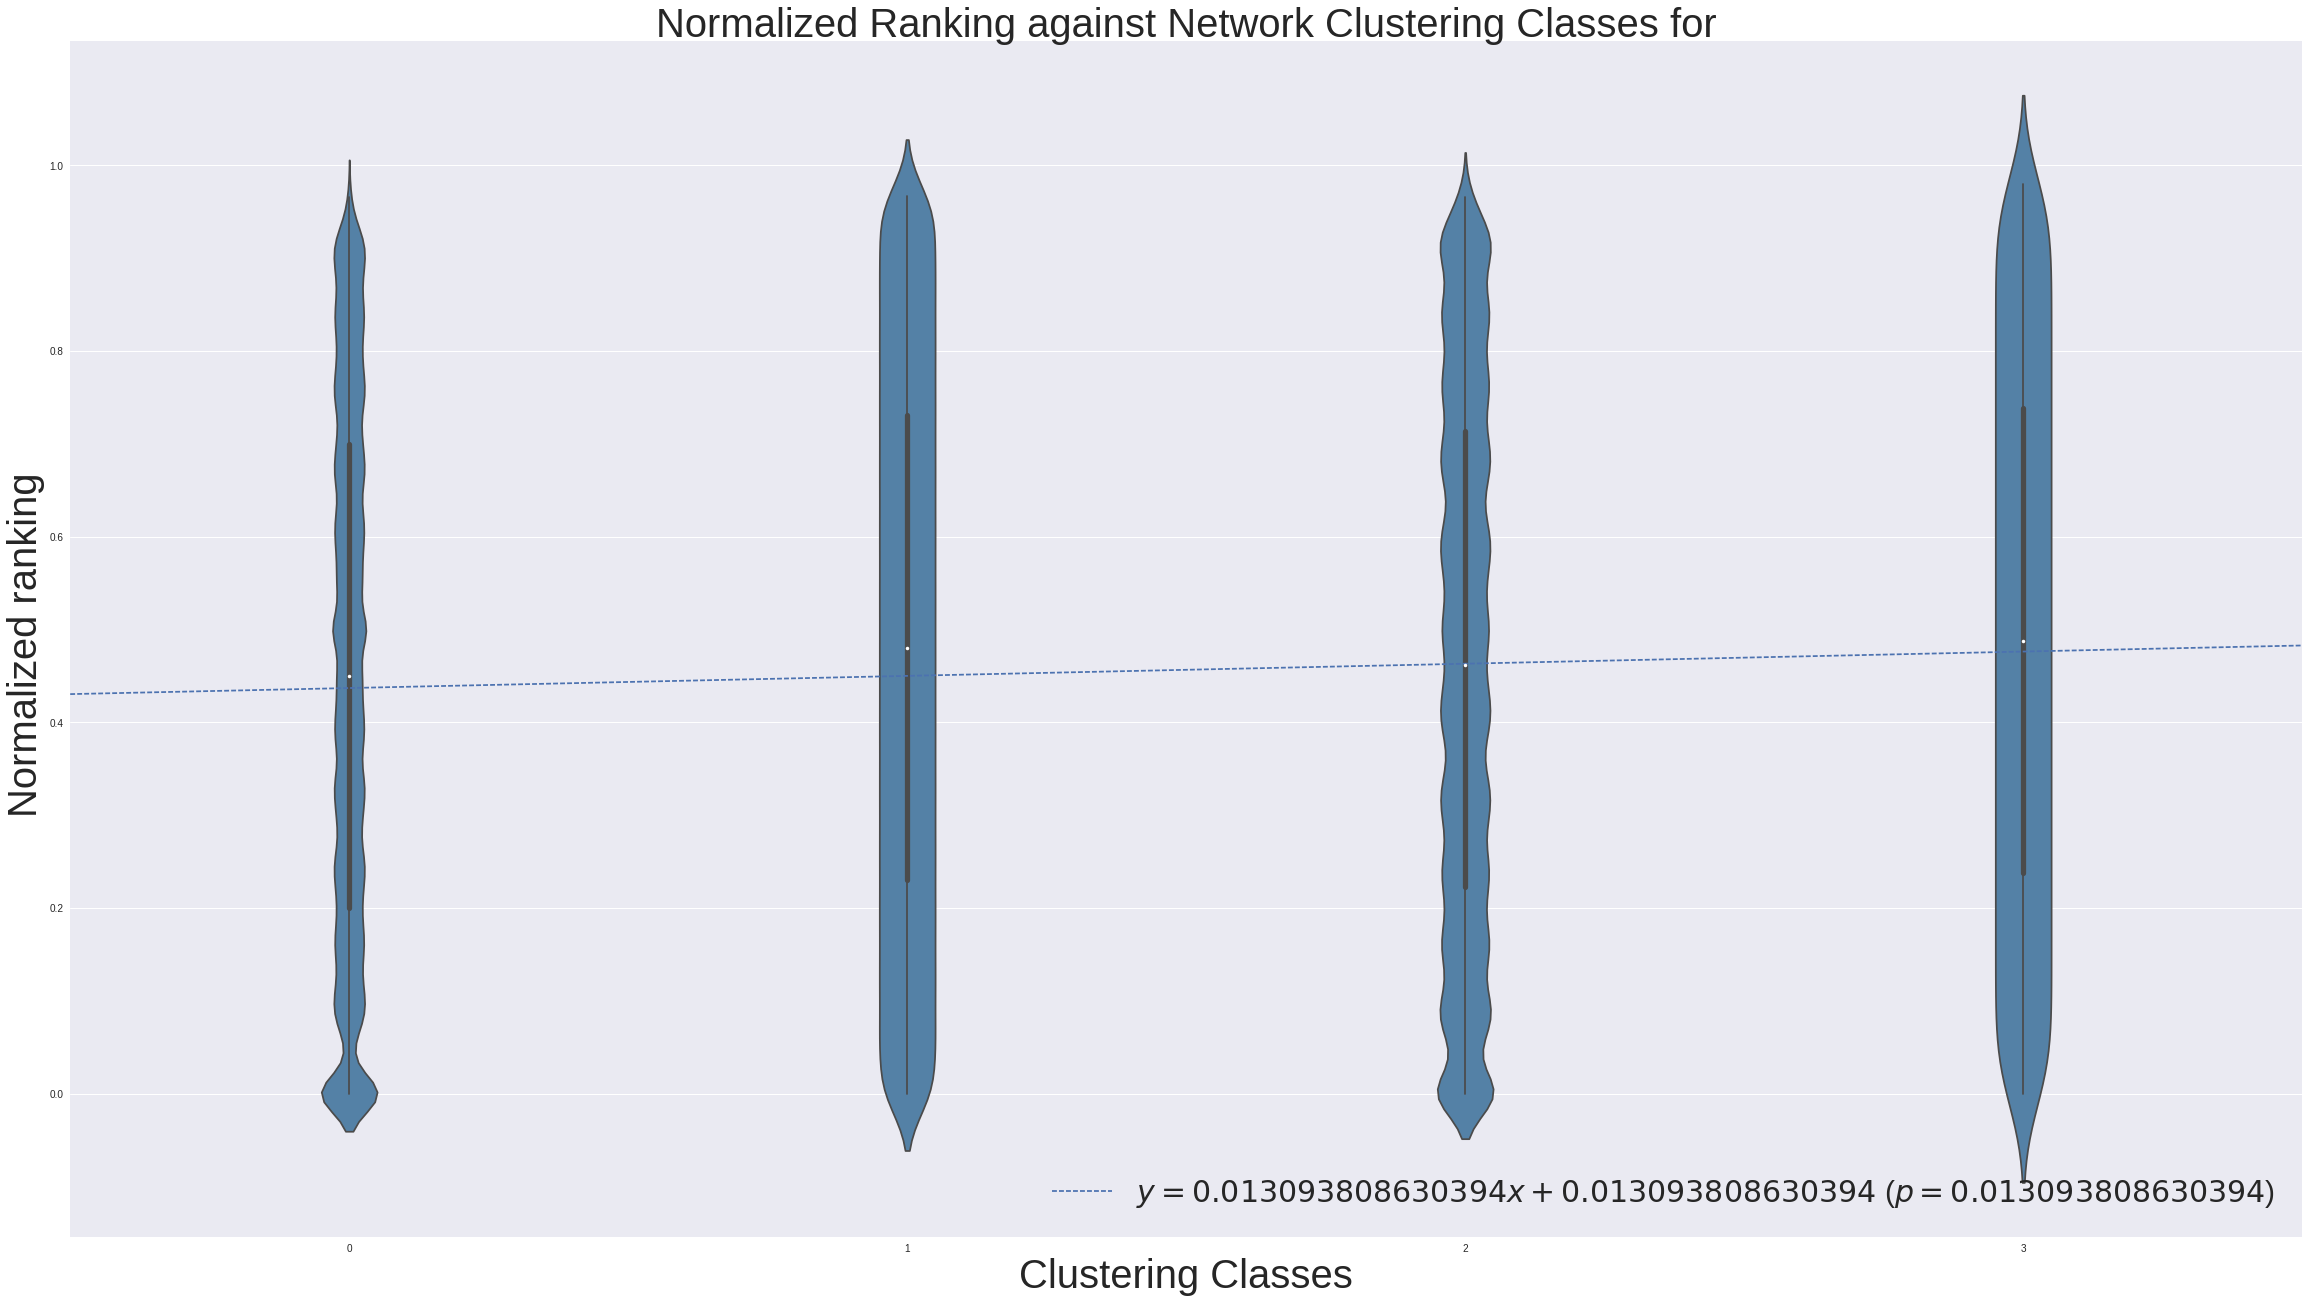
\includegraphics[width=1.2\linewidth,center]{chapter-four/normalized-rank-clusters.png}
	\caption{Violin plot of clusters against median normalized ranking}
	\label{fig:variation-clusters}
\end{figure}

In this subsection, PSO Gamber, Nydegger, Cautious QLearner, Gradual, have been
defined as the best performing strategies based on the median ranking.
Furthermore, the difference in the strategies normalized ranks have been studied,
based on groups of network clustering and connectivity. The results indicated
statistically significant difference. The effects of clustering and connectivity
coefficients will be analyzed in the following subsection by building regression
models.

\subsection{Regression}
This subsection concentrates, into build a regression model, for predicting
the normalized ranking of a strategy. This has been done, by identifying any
correlation between the topology measures and the participations of the strategy.
Initially, an analysis was performed for the entire data set, using the following
model.

\begin{align}
	\mathrm{normalised.ranking}_{t} = \alpha
	  & + \beta_{1}  \mathrm{average.neighborhood.score}_{t}          \\
	  & + \beta_{2}  \mathrm{normalized.average.score}_{t}            \\
	  & + \beta_{3}  \mathrm{cooperating.ratio}_{t}                   \\
	  & + \beta_{4}  \mathrm{connectivity}_{t}                        \\
	  & + \beta_{5}  \mathrm{clustering}_{t}                          \\
	  & + \beta_{6}  \mathrm{neighborhood.size}_{t}                   \\
	  & = \beta_{7}  \mathrm{tournament.size}_{t}                     \\
	  & + \beta_{8}  \mathrm{number.of.participations}_{t} + \epsilon
\end{align}

The result of the model are shown in Table~\ref{regression-complex-networks}.
All the predictors, expect clustering and neighborhood size, are significant.
Due their \(p\) value being less than 0.05.
Apart from normalized average score, connectivity and cooperating ratio, all
variables have a positive correlation with the normalized ranking. Because the
objective function, is to minimize the ranking, normalized average score,
connectivity and cooperating ratio are the only predictors affecting the performance
of a strategy positively. The model itself has a \(R\) square value of 0.006.

\begin{table}[!hbtp]
	\centering
	\begin{adjustbox}{width=0.7\textwidth}
		\small
		\begin{tabular}{llll}
			\toprule
			\multicolumn{4}{|c|}{\textbf{Regression Results}}         \\ \hline
			                           & coefficient & \(p\) value & \(R\) squared \\ \hline
			Intercept                  & 0.3712      & 0.000       & 0.006     \\ \hline
			average.neighborhood.score & 0.0206      & 0.000       & -         \\ \hline
			normalized.average.score   & -0.6150     & 0.001       & -         \\ \hline
			clustering                 & 0.0033      & 0.033       & -         \\ \hline
			connectivity               & -0.0011     & 0.000       & -         \\ \hline
			cooperating.ratio          & -0.0403     & 0.000       & -         \\ \hline
			tournament.size            & 0.0033      & 0.000       & -         \\ \hline
			frequency                  & 1.35e-06    & 0.000       & -         \\ \hline
			neighborhood.size          & 0.0005      & 0.017       & -         \\ \bottomrule

		\end{tabular}
	\end{adjustbox}
	\caption{Regression results}
	\label{regression-complex-networks}
	explaingn
\end{table}

The ability of the model to predict each of the 132 strategies has also been
tested. The results of each regression model in detail can be found in the
Appendix~\ref{append:reg-results-strategies}.

The results of implementing the models for each of the top ranking and the worst
ranking strategies are being discussed. The individual results of the best
performed strategies are shown in Table~\ref{reg-for-top}. The findings summarized
are the following,

\begin{itemize}
	\item PSO Gambler's, performance was significantly affected only by the tournament size
	\item Nydegger's, performance was significantly affected by clustering of the network,
	      the tournament size and the average neighborhood score
	\item Cautious QLearner's, performance was significantly affected by the tournament size,
	      the average neighborhood score and the normalized average score
	\item Gradual's, performance can not be predicted by the model
\end{itemize}

Overall, for each strategy the model had an low value of \(R\), thus there models
can only explain a small amount of variation in the normalized score of the strategies.
\begin{table}[!hbtp]
	\centering
	\begin{adjustbox}{width=1\textwidth, height=0.2\textwidth}
		\small
		\begin{tabular}{|l|l|l|l|l|l|l|l|l|l|l|l|l|}
			\toprule
			\multicolumn{13}{|c|}{\textbf{Regression Results}}                                                                       \\ \hline
			& \multicolumn{3}{l|}{PSO Gambler} & \multicolumn{3}{l|}{Nydegger} & \multicolumn{3}{l|}{Cautious QLearner} & \multicolumn{3}{l|}{Gradual} \\ \hline
			                           & coefficient  & \(p\) value & \(R\) squared & coefficient & \(p\) value & \(R\) squared & coefficient & \(p\) value & \(R\) squared & coefficient     & \(p\) value & \(R\) squared \\ \hline

			Intercept                  & 4.400080e-07 & 0.624059    & 0.070179      & 2.729e-09   & 0.269       & 0.042         & 1.508e-08   & 0.114       & 0.129         & 8.626e-08       & 0.058       & 0.020         \\ \hline
			average.neighborhood.score & -0.019826    & 0.863098    & -             & 0.0475      & 0.043       & -             & 0.1716      & 0.000       & -             & -0.0301         & 0.478       & -             \\ \hline
			normalized.average.score   & -28.609297   & 0.46898     & -             & 114.0857    & 0.163       & -             & -653.0862   & 0.000       & -             & 83.8451         & 0.339       & -             \\ \hline
			connectivity               & -0.007497    & 0.111566    & -             & -0.0019     & 0.316       & -             & 0.0043      & 0.110       & -             & 0.0006          & 0.838       & -             \\ \hline
			clustering                 & 0.104217     & 0.505338    & -             & -0.0749     & 0.004       & -             & -0.0594     & 0.059       & -             & -0.0108         & 0.785       & -             \\ \hline
			cooperating.ratio          & -0.081274    & 0.66987     & -             & 0.0456      & 0.331       & -             & 0.0673      & 0.497       & -             & -0.1310         & 0.082       & -             \\ \hline
			tournament.size            & 0.021194     & 0.000553    & -             & 0.0100      & 0.000       & -             & 0.0176      & 0.000       & -             & 0.0037          & 0.080       & -             \\ \hline
			frequency                  & 0.000268     & 0.624046    & -             & 4.884e-06   & 0.758       & -             & 3.942e-05   & 0.196       & -             & 0.0002          & 0.054       & -             \\ \hline
			neighborhood.size          & -0.003179    & 0.512211    & -             & 0.0004      & 0.844       & -             & -0.0066     & 0.033       & -             & 0.0005          & 0.894       & -             \\ \bottomrule

		\end{tabular}
	\end{adjustbox}
	\caption{Regression results for PSO Gambler, Nydegger, Cautious QLearner and Gradual}
	\label{reg-for-top}
\end{table}

Moreover, the results of the three worst ranking strategies are shown in Table~\ref{reg-for-bot}.
A summary of the results is as follows:
\begin{itemize}
	\item Meta Majority Finite Memory's performance was only significant affected by the tournament size
	\item Meta Minority's performance was only significant affected by the average neighborhood score
	      and the neighborhood size
	\item Limited Retaliate's (0.1/20) performance is significant affected by normalized average score,
	      cooperating ratio and  neighborhood size.
\end{itemize}

Similarly, each of the \(R\) square values is significant low. Thus, even if some
predictors were identified as statistically significant, due the low \(R\) square values
it is clear that the model can not predict the performance of either the top or low ranking strategies.

\begin{table}[!hbtp]
	\centering
	\begin{adjustbox}{width=1\textwidth, height=0.2\textwidth}
		\small
		\begin{tabular}{|l|l|l|l|l|l|l|l|l|l|l|l|l|}
			\toprule
			\multicolumn{10}{|c|}{\textbf{Regression Results}}                                                                       \\ \hline
			& \multicolumn{3}{l|}{Meta Majority Finite Memory} & \multicolumn{3}{l|}{Meta Minority} & \multicolumn{3}{l|}{Limited Retaliate (0.1/20)}\\ \hline
			                           & coefficient  & \(p\) value & \(R\) squared & coefficient   & \(p\) value & \(R\) squared & coefficient & \(p\) value  & \(R\) squared \\ \hline
			Intercept                  & 4.400080e-07 & 0.624059    & 0.070179      & -4.705709e-08 & 0.731064    & 0.037403      & 0.000002    & 2.461325e-18 & 0.103475      \\ \hline
			average.neighborhood.score & -0.019826    & 0.863098    & -             & 0.178246      & 0.001111    &               & -0.08878    & 0.19002      & -             \\ \hline
			normalized.average.score   & -28.609297   & 0.46898     & -             & 393.594243    & 0.074333    &               & -133.372492 & 0.000048     & -             \\ \hline
			connectivity               & -0.007497    & 0.111566    & -             & 0.002575      & 0.459493    &               & 0.009121    & 0.093335     & -             \\ \hline
			clustering                 & 0.104217     & 0.505338    & -             & 0.23341       & 0.029178    &               & -0.189418   & 0.109777     & -             \\ \hline
			cooperating.ratio          & -0.081274    & 0.66987     & -             & -0.631593     & 0.052838    &               & 0.346784    & 0.003463     & -             \\ \hline
			tournament.size            & 0.021194     & 0.000553    & -             & -0.002791     & 0.515109    &               & -0.03785    & 1.093118e-08 & -             \\ \hline
			frequency                  & 0.000268     & 0.624046    & -             & -0.000069     & 0.715793    &               & 0.002028    & 2.459952e-18 & -             \\ \hline
			neighborhood.size          & -0.003179    & 0.512211    & -             & -0.008742     & 0.014707    &               & 0.012772    & 0.019486     & -             \\ \bottomrule
		\end{tabular}
	\end{adjustbox}
	\caption{Regression results for ​Meta Majority Finite Memory, Meta Minority and Limited Retaliate (0.1/20)}
	\label{reg-for-bot}
\end{table}

Even so, the lowest ranked strategies have not been the strategies with the lowest
\(R\) square values. As it seems there have been other strategies to which their behavior
could not be predicted at all. These strategies were Davis, Soft Go By Majority: 10
and Contrite Tit For Tat. Their results after applying the regression model
can be seen in Table~\ref{reg-for-r-bot}.

\begin{table}[!hbtp]
	\centering
	\begin{adjustbox}{width=1\textwidth, height=0.2\textwidth}
		\small
		\begin{tabular}{|l|l|l|l|l|l|l|l|l|l|l|l|l|}
			\toprule
			\multicolumn{10}{|c|}{\textbf{Regression Results}}                                                                       \\ \hline
			& \multicolumn{3}{l|}{Davis} & \multicolumn{3}{l|}{Soft Go By Majority: 10} & \multicolumn{3}{l|}{Contrite Tit For Tat}\\ \hline
			  & coefficient & \(p\) value & \(R\) squared & coefficient & \(p\) value & \(R\) squared & coefficient & \(p\) value & \(R\) squared \\ \hline
			Intercept 								 &2.671044e-09  & 0.000355			& 0.002087	& 1.203656e-06	& 0.052384	& 0.003057	& -3.037859e-08 & 0.019441		 & 0.004457	\\ \hline
			average.neighborhood.score & 0.011477			& 0.210965			&	-					& -0.129346			& 0.272084 	& -					& 0.029967  		& 0.152437			& -         \\ \hline
			normalized.average.score	 & 8.706744			& 0.880304 			&	-					& 34.423987			& 0.836946 	& -					& 1364.800701 	& 0.005748			& -         \\ \hline
			connectivity							 & 0.000593			& 0.677547			&	-					& 0.005444			& 0.269910 	& -					& -0.000883			& 0.644392			& -         \\ \hline
			clustering  							 & 0.035832			& 0.005207			&	-					& -0.081300			& 0.606653	& -					& -0.030868 		& 0.117834			& -         \\ \hline
			cooperating.ratio					 & 0.007705			& 0.616883			&	-					& 0.030627 			& 0.944789 	& -					& -0.244267			& 0.017799			& -         \\ \hline
			tournament.size						 &-0.000044			& 0.948541			&	-					& -0.001665 		& 0.792195 	& -					& 0.004213 			& 0.000513			& -         \\ \hline
			frequency									 &0.000035			& 1.373152e-76	&	-					& 0.000919			& 5.214774e-02	& -			&  0.000002			& 8.786468e-01	& -         \\ \hline
			neighborhood.size			     &-0.001045			& 0.512251 			&	-					& -0.003463			& 0.487918			& -			& -0.000123 		& 0.954622	& -         		\\ \bottomrule
		\end{tabular}
	\end{adjustbox}
	\caption{Regression results for Davis, Soft Go By Majority: 10 and Contrite Tit For Tat}
	\label{reg-for-r-bot}
\end{table}

The only strategies that could be predicted by the model have been Fortress4 and
Once Bitten. For both strategies the model achieved a \(R\) square value of
0.80. Thus the model can explains 80 \% of the normalized rank variability for
each of the strategies. Results are given by Table~\ref{reg-for-r-top}.

\begin{table}[!hbtp]
	\centering
	\begin{adjustbox}{width=1\textwidth, height=0.2\textwidth}
		\small
		\begin{tabular}{|l|l|l|l|l|l|l|l|l|l|l|l|l|}
			\toprule
			\multicolumn{7}{|c|}{\textbf{Regression Results}}                                                                       \\ \hline
			&	\multicolumn{3}{l|}{Fortress4} & \multicolumn{3}{l|}{Once Bitten}\\ \hline
			  											   & coefficient & \(p\) value & \(R\) squared & coefficient & \(p\) value & \(R\) squared \\ \hline
			Intercept 								 & 7.664265e-01	& 6.883006e-01	& 0.800519	& 2.478012e-01 & 1.947868e-01 & 0.849582	\\ \hline
			average.neighborhood.score & 4.524753			& 8.618145e-01	& -					& 3.584271		 & 2.754952e-01	& -         \\ \hline
			normalized.average.score	 & -61.647292		& 3.363273e-01	& -					&-62.682017 	 & 3.283353e-01	& -         \\ \hline
			connectivity							 & -0.264150		& 6.877932e-01	& -					&-0.044507 		 & 3.574439e-01	& -         \\ \hline
			clustering  							 & 0.766427			& 6.883006e-01	& -					& 0.247801 		 & 1.947868e-01	& -         \\ \hline
			cooperating.ratio					 & -67.421175		& 5.575154e-01	& -					&-20.229438		 & 7.362663e-02	& -         \\ \hline
			tournament.size						 & 0.502277			& 6.893652e-01	& -					&0.203294  		 & 1.573032e-01	& -         \\ \hline
			frequency									 & 4.598559			& 6.883006e-01	& -					&2.230211  		 & 1.947868e-01	& -         \\ \hline
			neighborhood.size			   	 & -0.264150			& 0.687793		& -					&-0.044507 		 & 0.357444	& -         		\\ \bottomrule

		\end{tabular}
	\end{adjustbox}
	\caption{Regression results for ​Fool Me Forever, Fortress4 and Once Bitten}
	\label{reg-for-r-top}
\end{table}

In this subsection, the performance of the strategies has been tried to be predicted
by a regression model. The results, for running this regression model to the
hole data set returned that cooperating ratio, connectivity and the normalized
average score were significant predictors. Furthermore, by analyzing each strategy
individual to test whether their behavior can be predicted, returned that this
is possible for only 2 of the 132 strategies. For the rest, their performance can not
be accurately predicted by the possible predictors given. In the next section,
a summary of the findings of this chapter have been stated.

\section{Summary}
In this chapter, experiments with more complex networks topologies have been
performed. Various networks have been considered: all with a varying topological
structure, obtained using methods to create random, small world and complete networks.

The methods have been individual discussed and an overview of the data they
produced has been implemented. To be able to perform analysis on the data set
produced by using this methods, two classification have been conducted.
In this chapter, a new measure has been used, the normalized median rank.
The four top performed strategies of the complex networks experiment have
been named. PSO Gamblre, Nydegger, Cautious QLearner and Gradual.

An analysis of the normalized ranking was then conducted. The findings are the
following. Normalized ranking, for the top strategies have been significantly different
between groups of connectivity, clustering and cooperating. Also cooperating behavior, has been showed to
be affecting the performance. All three strategies have been characterized as highly
cooperators by the analysis in ~\autoref{sub:classification}. Regression showed that,
predicting the performance of the strategies is possible of 2 of the 132 strategies.
Even so, this could be further investigated.

In conclusion, further research with more data and different random topology
is needed. Thought connectivity and cooperating ratio seems to have played a role,
there is not enough validation in the results. The topology does in did affect
the strategies, but a strategy that could outperform any topology has now been
found yet. Whether a strategy like this exist or not in the Axelrod-Python Library
is not sure. Thus, in the following chapter a strategy will be trained.
% miyagi
